% ==============================================================================
% MODELO UNINOVE (PPGI/PPGP): PRÉ-QUALIFICAÇÃO, QUALIFICAÇÃO E DEFESA
% Conforme o Manual de Orientação para Apresentação de Trabalhos Acadêmicos
% do Sistema de Bibliotecas Prof. José Storópoli (março de 2025).
%
% Estrutura de pastas:
%   config/        dados do trabalho e preâmbulo complementar
%   pre-textuais/  resumo, abstract, listas e elementos opcionais
%   capitulos/     um arquivo por capítulo
%   pos-textuais/  declaração de IA e referências (.bib)
%   apendices/     documentos elaborados pelo autor
%   anexos/        documentos de terceiros
%   figuras/       imagens (png, pdf, jpg) e figuras/tikz/ para diagramas
% ==============================================================================

% ------------------------------------------------------------------------------
% 1. OPÇÕES DE CITAÇÃO (antes da classe)
% 'abnt-citacao-minuscula': sobrenome em minúsculas, inclusive entre
%   parênteses, como exige a NBR 10520:2023: (Silva, 2024); ver config/abnt-opcoes.bib
% 'abnt-etal-cite=3': et al. somente a partir de 4 autores (NBR 10520:2023)
% 'abnt-etal-text=emph': et al. em itálico
% 'abnt-emphasize=bf': destaque em negrito no título da obra ou do periódico
%   (manual, cap. 4, item 1.1.1)
% ------------------------------------------------------------------------------
\PassOptionsToPackage{abnt-citacao-minuscula,abnt-etal-cite=3,abnt-etal-text=emph,abnt-emphasize=bf}{abntex2cite}
\PassOptionsToPackage{table}{xcolor}

\documentclass{uninove-ppgi}

% ------------------------------------------------------------------------------
% 2. MODO DE COMPILAÇÃO
% [revisao]: notas, marcações, lista de pendências e carimbo de versão
% [final]  : texto limpo, em preto, para envio à banca ou depósito
% ------------------------------------------------------------------------------
\usepackage[revisao]{revisao}

% ------------------------------------------------------------------------------
% 3. PREÂMBULO COMPLEMENTAR E DADOS DO TRABALHO
% ------------------------------------------------------------------------------
% ==============================================================================
%  PREÂMBULO COMPLEMENTAR (config/preambulo.tex)
% ==============================================================================
%
%  O que este arquivo faz
%    Carrega pacotes e define estilos e comandos usados no texto: tabelas,
%    caixas de destaque, diagramas, listagens de código e cores dos links.
%
%  O que este arquivo NÃO faz
%    A formatação ABNT (margens, fonte, espaçamento, títulos, listas, sumário,
%    referências) está na classe uninove-ppgi.cls. Não a altere aqui.
%
%  Ordem de carregamento (definida em main.tex)
%    1. classe uninove-ppgi.cls
%    2. pacote revisao.sty      (define \ifmodofinal, usado na Seção 6 abaixo)
%    3. este arquivo
%    4. config/dados.tex
%
%  Antes de acrescentar um pacote, verifique se ele já não é carregado pela
%  classe (pacotes repetidos com opções diferentes geram erro "option clash").
%
%  Sumário deste arquivo
%    1. Tabelas e posicionamento de flutuantes
%    2. Atalhos e comandos auxiliares
%    3. Caixas de destaque e de orientação ao aluno
%    4. Diagramas em TikZ
%    5. Listagens de código e expressões de busca
%    6. Cores dos links conforme o modo de compilação
% ==============================================================================


% ==============================================================================
%  1. TABELAS E POSICIONAMENTO DE FLUTUANTES
% ==============================================================================

% float: habilita a opção [H], que fixa figuras, quadros e tabelas
% exatamente no ponto do texto em que foram escritos.
%   Uso: \begin{figure}[H] ... \end{figure}
\usepackage{float}

% longtable: tabelas que continuam na página seguinte.
%   Uso: \begin{longtable}{...} ... \end{longtable}
%   (não deve ser colocada dentro de \begin{table})
\usepackage{longtable}

% Observação: xcolor, colortbl, tabularx, booktabs, multirow e makecell já são
% carregados pela classe. A opção [table] do xcolor é repassada em main.tex.


% ==============================================================================
%  2. ATALHOS E COMANDOS AUXILIARES
% ==============================================================================

% \mes: preenche de cinza uma célula do cronograma (Capítulo 5).
%   Uso: 1 & Atividade & \mes & \mes & & \\ \hline
\newcommand{\mes}{\cellcolor{black!55}}


% ==============================================================================
%  3. CAIXAS DE DESTAQUE E DE ORIENTAÇÃO AO ALUNO
% ==============================================================================

% tcolorbox e mdframed: pacotes para caixas com moldura e fundo colorido.
\usepackage[most]{tcolorbox}
\usepackage{mdframed}

% ------------------------------------------------------------------------------
% Ambiente "destaque": caixa com fundo cinza claro e filete à esquerda.
% Quebra de página automaticamente, se necessário.
%   Uso: \begin{destaque} texto \end{destaque}
% ------------------------------------------------------------------------------
\newmdenv[
  linecolor=gray!50, linewidth=0.4pt,           % cor e espessura do filete
  leftline=true, rightline=false,               % filete apenas à esquerda
  topline=false, bottomline=false,
  backgroundcolor=gray!5,                       % fundo cinza bem claro
  innerleftmargin=10pt, innerrightmargin=6pt,   % espaçamento interno
  innertopmargin=6pt, innerbottommargin=6pt,
  skipabove=\baselineskip, skipbelow=\baselineskip  % espaço antes e depois
]{destaque}

% ------------------------------------------------------------------------------
% Ambiente "orientacao": caixa com instruções ao aluno.
% Aparece no PDF apenas no modo [revisao]; no modo [final], o conteúdo é
% descartado automaticamente, sem necessidade de apagá-lo do código.
%   Uso: \begin{orientacao}[Título opcional]
%          Texto da orientação.
%        \end{orientacao}
% Depende do ambiente "destaque" (acima) e de \ifmodofinal (revisao.sty).
% ------------------------------------------------------------------------------
\ifmodofinal
  % Modo final: tudo entre \begin{orientacao} e \end{orientacao} é ignorado
  \newenvironment{orientacao}[1][]{\comment}{\endcomment}
\else
  % Modo revisão: caixa de destaque com o título "Orientação ao aluno"
  \newenvironment{orientacao}[1][]
  {\begin{destaque}\small\setlength{\parindent}{0pt}%
      \textbf{Orientação ao aluno\if\relax\detokenize{#1}\relax\else: #1\fi.}%
      \par\smallskip}
      {\end{destaque}}
\fi


% ==============================================================================
%  4. DIAGRAMAS EM TIKZ
% ==============================================================================

% Bibliotecas do TikZ (o pacote tikz já é carregado pela classe):
%   shapes.geometric  formas geométricas (losangos, elipses etc.)
%   arrows.meta       pontas de seta configuráveis
%   positioning       posicionamento relativo (below=of, right=of)
%   fit               caixas que envolvem outros nós
%   calc              cálculos com coordenadas
\usetikzlibrary{shapes.geometric, arrows.meta, positioning, fit, calc}

% Estilos padronizados para fluxogramas e desenhos da pesquisa.
%   Uso: \node[box] (a) {Etapa 1};
%        \node[box, below=of a] (b) {Etapa 2};
%        \draw[arrow] (a) -- (b);
\tikzset{
% box: caixa principal, arredondada, sem hifenização no texto interno
box/.style={
    draw, rectangle, rounded corners=4pt,
    minimum width=9cm, minimum height=1.0cm, text width=6.8cm,
    align=center, font=\small, inner sep=6pt, fill=white,
    execute at begin node={\hyphenpenalty=10000\exhyphenpenalty=10000}
  },
% srcbox: caixa compacta, para fontes de dados no topo de um diagrama
srcbox/.style={
    draw, rectangle, rounded corners=4pt,
    minimum width=3.2cm, minimum height=1.4cm, text width=2.9cm,
    align=center, font=\small, inner sep=8pt, fill=white,
    execute at begin node={\hyphenpenalty=10000\exhyphenpenalty=10000}
  },
% arrow: conector com ponta Stealth de 6 pt
arrow/.style={
-{Stealth[length=6pt, width=5pt]},
line width=0.8pt
}
}


% ==============================================================================
%  5. LISTAGENS DE CÓDIGO E EXPRESSÕES DE BUSCA
% ==============================================================================

% upquote: mantém as aspas retas (") nas listagens, em vez de aspas curvas.
% Essencial para que expressões de busca copiadas do PDF funcionem nas bases.
\usepackage{upquote}

% ------------------------------------------------------------------------------
% Estilo "codigo": trechos de programa, com numeração de linhas e cores.
%   Uso: \begin{lstlisting}[style=codigo, language=Python]
%          ...código...
%        \end{lstlisting}
%   Linguagens comuns: Python, R, SQL, Java, C, [LaTeX]TeX.
% ------------------------------------------------------------------------------
\lstdefinestyle{codigo}{
  basicstyle=\footnotesize\ttfamily,           % fonte monoespaçada pequena
  keywordstyle=\color{blue}\bfseries,          % palavras reservadas
  commentstyle=\color{green!50!black},         % comentários
  stringstyle=\color{red},                     % textos entre aspas
  numbers=left, numberstyle=\tiny, numbersep=5pt,  % numeração das linhas
  frame=single, rulecolor=\color{gray},        % moldura
  xleftmargin=20pt, framexleftmargin=15pt,     % recuo para a numeração
  tabsize=3,
  breaklines=true,                             % quebra linhas longas
  showstringspaces=false                       % não marca espaços em textos
}

% ------------------------------------------------------------------------------
% Estilo "busca": expressões de busca em bases de dados (Apêndice A).
% Preserva aspas retas, quebras de linha e recuos, de modo que a expressão
% possa ser copiada do PDF e colada na base sem alterações.
%   Uso: \begin{lstlisting}[style=busca]
%          TITLE-ABS-KEY("termo 1" AND "termo 2")
%        \end{lstlisting}
% ------------------------------------------------------------------------------
\lstdefinestyle{busca}{
basicstyle=\footnotesize\ttfamily,
frame=single, rulecolor=\color{black},
breaklines=true, breakatwhitespace=true,     % quebra apenas em espaços
columns=fullflexible, keepspaces=true,       % espaçamento natural
showstringspaces=false, upquote=true,        % aspas retas
% Acentos dentro das listagens (o listings não os reconhece sozinho)
inputencoding=utf8, extendedchars=true,
literate={á}{{\'a}}1 {é}{{\'e}}1 {í}{{\'i}}1 {ó}{{\'o}}1 {ú}{{\'u}}1
{ã}{{\~a}}1 {õ}{{\~o}}1 {ç}{{\c{c}}}1 {â}{{\^a}}1 {ê}{{\^e}}1
}


% ==============================================================================
%  6. CORES DOS LINKS CONFORME O MODO DE COMPILAÇÃO
% ==============================================================================
% O modo é escolhido em main.tex: \usepackage[revisao]{revisao} ou [final].
%
%   Modo revisão: links em azul (facilita a navegação durante a orientação)
%                 e indicação "Citado na pág." após cada referência, que
%                 revela obras listadas mas não citadas no texto.
%   Modo final:   todo o texto em preto, como exige o manual da biblioteca,
%                 e sem a indicação "Citado na pág.", que não é ABNT.
% ------------------------------------------------------------------------------
\ifmodofinal
  \hypersetup{colorlinks=true, linkcolor=black, citecolor=black,
    filecolor=black, urlcolor=black}
  \renewcommand*{\backrefalt}[4]{}             % remove "Citado na pág."
\else
  \hypersetup{colorlinks=true, linkcolor=blue, citecolor=blue,
    filecolor=blue, urlcolor=blue}
\fi

% ==============================================================================
%  7. METADADOS DO PDF (Arquivo > Propriedades no leitor de PDF)
% ==============================================================================
% Preenchidos automaticamente; não é preciso editar nada aqui.
%   Título, autor e assunto: campos de config/dados.tex
%   Palavras-chave: \PalavrasChave de pre-textuais/resumo.tex
% Como o resumo é lido depois da primeira página, as palavras-chave são
% guardadas no arquivo .aux e gravadas no PDF na compilação seguinte
% (o latexmk e o LaTeX Workshop já compilam mais de uma vez).
% ------------------------------------------------------------------------------
\makeatletter
\providecommand{\pdf@palavraschave}{}
\AtBeginDocument{%
  \hypersetup{
    pdftitle    = {\titulo},
    pdfauthor   = {\autor},
    pdfsubject  = {\tipoexame\ -- \siglaprograma, Universidade Nove de Julho (\ano)},
    pdfkeywords = {\pdf@palavraschave},
    pdfcreator  = {\autor}
  }%
}
\AtEndDocument{%
  \ifdefined\palavraschave
    \immediate\write\@auxout{%
      \gdef\string\pdf@palavraschave{\unexpanded\expandafter{\palavraschave}}}%
  \fi}
\makeatother
% ==============================================================================
% DADOS DO TRABALHO (capa, folha de rosto e folha de aprovação)
% Único arquivo que o(a) aluno(a) precisa editar na abertura do projeto.
% ==============================================================================

\Universidade{UNIVERSIDADE NOVE DE JULHO -- UNINOVE}
\Programa{PROGRAMA DE PÓS-GRADUAÇÃO EM INFORMÁTICA E GESTÃO DO CONHECIMENTO -- PPGI}
% Para o PPGP, descomentar e ajustar também a linha \Programa acima:
% \Area{Gestão de Projetos}
% \SiglaPrograma{PPGP}

\Autor{NOME COMPLETO DO(A) AUTOR(A)} % também usado na legenda de revisores (revisao.sty)
\Titulo{TÍTULO DO TRABALHO: SUBTÍTULO (SE HOUVER)}

\Tipoexame{Pré-Qualificação} % Pré-Qualificação, Qualificação ou Defesa
\Titulacao{Mestre}           % Mestre, Mestra, Doutor ou Doutora

% Os nomes abaixo aparecem na capa, na folha de rosto, na folha de aprovação
% e na legenda de revisores do modo revisão (revisao.sty).
\Orientador{Prof. Dr. Nome do Orientador} % obrigatório
\Coorientador{Prof. Dr. Nome do Coorientador} % opcional: comentar se não houver
% \Disciplina{Seminários em Tecnologia da Informação Inteligente} % opcional (somente pré-qualificação)
\Ingresso{03/2026}                    % opcional
% \Linha{LP1 -- Modelagem e Otimização Computacional}   % opcional
\Linha{LP2 -- Sistemas Inteligentes}   % opcional
% \Linha{Gestão da Tecnologia da Informação e Conhecimento}   % opcional
\Ano{2027}

% ------------------------------------------------------------------------------
% Somente na Defesa (folha de aprovação; ativar \folhaaprovacao em main.tex)
% ------------------------------------------------------------------------------
% \DataAprovacao{dia mês e ano} % obrigatório na Defesa
% \MembroBanca{\orientador}{Universidade Nove de Julho -- Orientador}
% \MembroBanca{\coorientador}{Instituição -- Membro interno}
% \MembroBanca{Prof(a). Dr(a). Nome}{Instituição -- Membro externo}

% ------------------------------------------------------------------------------
% Rótulo exibido no carimbo do modo revisão (atualizar a cada entrega)
% ------------------------------------------------------------------------------
\versaodocumento{\tipoexame, v1}


% ------------------------------------------------------------------------------
% 4. ADAPTAÇÃO AUTOMÁTICA À ETAPA (definida por \Tipoexame em config/dados.tex)
% Pré-Qualificação e Qualificação: capítulo 4 "Resultados preliminares" e
%   capítulo 5 "Planos para a continuidade do trabalho".
% Defesa: capítulo 4 "Resultados e discussão" e capítulo 5 "Conclusão".
% ------------------------------------------------------------------------------
\newif\ifdefesa
\ifthenelse{\equal{\tipoexame}{Defesa}}{\defesatrue}{\defesafalse}
\ifdefesa
  \newcommand{\titresultados}{Resultados e discussão}
\else
  \newcommand{\titresultados}{Resultados preliminares}
\fi

% Compilar apenas alguns capítulos (acelera a edição; descomentar e ajustar)
% \includeonly{capitulos/03-metodologia}

\begin{document}

% ==============================================================================
% ELEMENTOS PRÉ-TEXTUAIS
% Folhas contadas a partir da folha de rosto, sem número impresso.
% Ordem: NBR 14724:2024
% ==============================================================================
\pretextual

% Lista de notas de revisão em aberto (desaparece no modo final)
\listadenotas

\capa                                   % obrigatório
\folharosto                             % obrigatório (folha 1)

% Descomentar as linha abaixo apenas na versão final, após a Defesa
% \fichacatalografica{pre-textuais/ficha-catalografica.pdf} 
% \folhaaprovacao

% ==============================================================================
% ELEMENTOS Opcionais.
% Descomentar as linhas abaixo apenas na versão final, após a Defesa
% ==============================================================================
% % ==============================================================================
% DEDICATÓRIA (opcional; manual, cap. 2, item 6)
% - Não tem título: a palavra "Dedicatória" NÃO aparece na página.
% - Vem logo após a folha de aprovação (ou após a folha de rosto, na
%   qualificação), em folha própria, sem número impresso.
% - Texto breve, de uma a três linhas, em tom pessoal e sóbrio.
% - Dedica-se o trabalho a pessoas; agradecimentos a instituições, ao
%   orientador e a agências de fomento vão na seção de Agradecimentos.
% - Se não houver dedicatória, manter a linha comentada em main.tex.
% ==============================================================================
\begin{dedicatoria}
  Aos meus pais, \preencher{nomes}, que me ensinaram o valor do estudo
  muito antes de eu compreendê-lo.

  \vspace{1em}
  À \preencher{nome}, pela paciência e pelo apoio em cada etapa desta jornada.
\end{dedicatoria}      % opcional
% % ==============================================================================
% AGRADECIMENTOS (opcional; manual, cap. 2, item 7)
% - Título "AGRADECIMENTOS" centralizado e em negrito (gerado pela classe).
% - Vem após a dedicatória (ou após a folha de aprovação, se não houver
%   dedicatória), em folha própria, sem número impresso.
% - Texto em parágrafos normais, com recuo. Não usar \noindent nem \newline
%   para separar parágrafos: basta deixar uma linha em branco entre eles.
% - Ordem sugerida: orientação, banca, docentes, colegas, instituição e
%   agências de fomento, família e amigos. A ordem é livre, mas convém
%   manter as menções institucionais juntas.
% - Tom pessoal, porém sóbrio. Evitar exageros, piadas internas e listas
%   extensas de nomes. Uma página costuma ser suficiente.
% - Usar o tratamento correto de cada pessoa: Prof. Dr. / Profa. Dra.
% - Apagar os parágrafos que não se aplicam e todos os campos \preencher.
% ==============================================================================
\begin{agradecimentos}

  % --- Orientação ---------------------------------------------------------------
  % Mencionar contribuições concretas (rigor, disponibilidade, autonomia),
  % e não apenas elogios genéricos.
  Ao meu orientador, \preencher{Prof. Dr. nome completo}, pela orientação
  criteriosa, pela confiança e pelas contribuições decisivas ao desenvolvimento
  deste trabalho.

  % Excluir se não houver coorientação.
  Ao meu coorientador, \preencher{Prof. Dr. nome completo}, pelas sugestões
  e pelo acompanhamento ao longo da pesquisa.

  % --- Banca e docentes ---------------------------------------------------------
  % Na versão de Defesa, agradecer aos membros da banca de qualificação, cujas
  % recomendações foram incorporadas ao texto.
  Aos professores \preencher{nomes}, membros da banca de qualificação, pelas
  recomendações que aprimoraram esta \preencher{dissertação ou tese}.

  % Pode ser geral ou nominal; se nominal, citar poucos nomes e justificar.
  Aos docentes do Programa de Pós-Graduação em \preencher{Informática e Gestão
    do Conhecimento ou Gestão de Projetos}, pelo conhecimento compartilhado
  nas disciplinas e seminários.

  % --- Colegas ------------------------------------------------------------------
  Aos colegas do \preencher{grupo de pesquisa ou turma}, pela troca de ideias
  e pelo apoio mútuo.

  % --- Instituição e fomento ----------------------------------------------------
  % Bolsistas FAP/UNINOVE:
  Agradeço à Universidade Nove de Julho (UNINOVE) pela concessão da bolsa de
  estudos do Fundo de Apoio à Pesquisa (FAP).

  % Outras agências: atenção à crase (à CAPES, à FAPESP, mas ao CNPq) e ao
  % número do processo, exigido pelo CNPq e pelas fundações estaduais.
  Agradeço \preencher{à CAPES, ao CNPq ou à agência de fomento} pela
  concessão \preencher{da bolsa de estudos ou da taxa}
  (processo n.\textsuperscript{o}~\preencher{número}).

  % Bolsistas CAPES: frase OBRIGATÓRIA (Portaria CAPES n.º 206/2018), com
  % esta redação exata. Descomentar se aplicável.
  % O presente trabalho foi realizado com apoio da Coordenação de
  % Aperfeiçoamento de Pessoal de Nível Superior -- Brasil (CAPES) --
  % Código de Financiamento 001.

  % --- Família e amigos --------------------------------------------------------
  À minha família, especialmente \preencher{nomes}, pelo apoio incondicional
  e pela compreensão nos momentos de ausência.

  % --- Fechamento ---------------------------------------------------------------
  Por fim, agradeço a todos que, direta ou indiretamente, contribuíram para a
  realização deste trabalho.

\end{agradecimentos}   % opcional
% % ==============================================================================
% EPÍGRAFE (opcional; manual, cap. 2, item 8)
% - Não tem título: a palavra "Epígrafe" NÃO aparece na página.
% - Vem após os agradecimentos, em folha própria, sem número impresso.
% - É uma citação direta e segue a NBR 10520:2023: aspas duplas, autor em
%   minúsculas, ano e página (quando houver). Texto traduzido pelo autor
%   leva a indicação "tradução nossa".
% - A obra citada DEVE constar nas Referências, na edição efetivamente
%   consultada. Não usar frases de autoria incerta, comuns na internet.
% - Preferir citações relacionadas ao tema ou ao espírito da pesquisa.
% - A NBR 14724 também admite epígrafes na abertura de cada capítulo.
% ==============================================================================
\begin{epigrafe}
  ``Se vi mais longe, foi por estar sobre os ombros de gigantes.''

  \vspace{0.5em}
  \hfill (Newton, 1676, tradução nossa)
\end{epigrafe}

% Exemplo de referência correspondente (adaptar à edição consultada):
% NEWTON, Isaac. [Carta a Robert Hooke, 5 fev. 1676]. In: TURNBULL, H. W.
% (ed.). The correspondence of Isaac Newton. Cambridge: Cambridge University
% Press, 1959. v. 1, p. 416.         % opcional

% Elementos obrigatórios
% ==============================================================================
% RESUMO (obrigatório; NBR 6028:2021)
% Parágrafo único, voz ativa, terceira pessoa do singular, 150 a 500 palavras,
% sem citações. Palavras-chave: 3 a 6, separadas por ponto e vírgula, em
% minúsculas (exceto nomes próprios e científicos) e finalizadas por ponto.
% Vocabulário controlado: https://acervo.bn.gov.br/sophia_web
% ==============================================================================
\PalavrasChave{palavra-chave 1; palavra-chave 2; palavra-chave 3; palavra-chave 4; palavra-chave 5.}

\begin{resumo}
  \noindent Aqui vai o resumo do trabalho, que deve conter entre 150 e 500 palavras. O resumo deve apresentar de forma concisa o contexto, o objetivo, a metodologia e os resultados (parciais, na qualificação) do trabalho. Deve ser escrito em parágrafo único, sem citações ou referências bibliográficas.
\end{resumo}
             % obrigatório
% ==============================================================================
% ABSTRACT (obrigatório; mesmo formato do resumo, em página seguinte)
% ==============================================================================
\KeyWords{keyword 1; keyword 2; keyword 3; keyword 4; keyword 5.}

\begin{abstract}
  \noindent English version of the abstract, faithful to the Portuguese text, with the same structure and length.
\end{abstract}
           % obrigatório
% ==============================================================================
% LISTAS DE ILUSTRAÇÕES E TABELAS (opcionais; NBR 14724:2024)
% Com mais de um tipo de ilustração, recomenda-se uma lista própria para cada
% tipo (figuras, quadros). Remover a lista de um tipo que não ocorra no texto.
% Os itens seguem o formato: Figura 1 – Título ..... página
% ==============================================================================
\listoffigures
\listofquadros
\listoftables

% Lista de algoritmos (opcional)
% \listofalgorithms
             % figuras, tabelas e quadros
% ==============================================================================
% LISTA DE ABREVIATURAS E SIGLAS (opcional; NBR 14724:2024)
% - Ordem ALFABÉTICA.
% - Incluir apenas as siglas efetivamente usadas no texto. Na primeira
%   ocorrência, a sigla vem entre parênteses, após o nome por extenso:
%   "Comitê de Ética em Pesquisa (CEP)". Depois, usa-se só a sigla.
% - Siglas estrangeiras: por extenso no idioma original, em itálico, e,
%   se útil, a tradução entre parênteses.
% - Não entra no sumário.
% ==============================================================================
\begin{listaabreviaturas}
  CEP    & Comitê de Ética em Pesquisa \\
  CNS    & Conselho Nacional de Saúde \\
  CONEP  & Comissão Nacional de Ética em Pesquisa \\
  IA     & Inteligência Artificial \\
  IAGen  & Inteligência Artificial Generativa \\
  OSF    & \textit{Open Science Framework} \\
  POC    & Prova de conceito (\textit{proof of concept}) \\
  PRISMA & \textit{Preferred Reporting Items for Systematic Reviews and Meta-Analyses} \\
  SHAP   & \textit{SHapley Additive exPlanations} \\
  XAI    & \textit{Explainable Artificial Intelligence} (Inteligência Artificial Explicável) \\
\end{listaabreviaturas}

% ==============================================================================
% LISTA DE SÍMBOLOS (opcional; NBR 14724:2024)
% - Ordem em que os símbolos APARECEM NO TEXTO (e não alfabética).
% - Cada símbolo com o seu significado; um símbolo, um único significado em
%   todo o trabalho (por isso a partição de validação usa o índice m, e não
%   j, já reservado ao jogador/variável na Equação 2.1).
% - Atualizar sempre que uma equação for incluída, alterada ou removida.
% - Não entra no sumário.
% - Cada linha: \simbolo{símbolo}{significado}. O comando não usa tabela,
%   o que evita conflitos de pacotes com colunas de largura fixa.
% ==============================================================================
\providecommand{\simbolo}[2]{%
  \noindent\parbox[t]{2.2cm}{#1}\parbox[t]{13.2cm}{#2}\par\smallskip}

\begin{listasimbolos}
  \simbolo{$j$}{Índice de um jogador (variável preditora)}
  \simbolo{$\phi_j(v)$}{Valor de Shapley do jogador $j$}
  \simbolo{$v$}{Função característica, que associa a cada coalizão o seu ganho}
  \simbolo{$S$}{Coalizão de jogadores que não contém $j$}
  \simbolo{$N$}{Conjunto de jogadores (variáveis preditoras)}
  \simbolo{$|N|$}{Cardinalidade do conjunto $N$ (número de elementos)}
  \simbolo{$VP$}{Número de verdadeiros positivos}
  \simbolo{$FP$}{Número de falsos positivos}
  \simbolo{$FN$}{Número de falsos negativos}
  \simbolo{$\tau$}{Limiar de decisão do classificador}
  \simbolo{$\hat{p}_i$}{Probabilidade estimada da classe positiva para a observação $i$}
  \simbolo{$i$}{Índice de uma observação}
  \simbolo{$F_1$}{Média harmônica entre precisão e revocação (\textit{F1-score})}
  \simbolo{$\theta$}{Vetor de hiperparâmetros de um modelo}
  \simbolo{$k$}{Número de partições da validação cruzada}
  \simbolo{$\hat{\theta}$}{Hiperparâmetros selecionados por validação cruzada}
  \simbolo{$\argmin$}{Argumento que minimiza a expressão}
  \simbolo{$\Theta$}{Espaço de busca dos hiperparâmetros}
  \simbolo{$\mathcal{L}$}{Função de perda}
  \simbolo{$D_m$}{$m$-ésima partição de validação}
  \simbolo{$m$}{Índice de uma partição de validação}
\end{listasimbolos}
       % opcional
\tableofcontents                        % obrigatório; último elemento pré-textual

% ==============================================================================
% ELEMENTOS TEXTUAIS OBRIGATÓRIOS (numeração impressa a partir da Introdução)
% ==============================================================================
\textual

% ==============================================================================
% CAPÍTULO 1: INTRODUÇÃO
% Títulos de seção: apenas a primeira letra em maiúscula (manual, item 2)
% ==============================================================================
\chapter{Introdução}
\label{ch:introducao}

\section{Contextualização}
\label{sec:contextualizacao}
A contextualização tem por finalidade situar o leitor no macrocenário temático em que a pesquisa se insere, apresentando as circunstâncias históricas, conceituais, práticas ou tecnológicas que envolvem o objeto de estudo. Sua função estrutural é traçar um panorama abrangente que evidencie a relevância da área de investigação e a dinâmica atual do campo científico ou de mercado. Ela estabelece as bases conceituais iniciais e o pano de fundo necessário para que a emergência do problema de pesquisa seja compreendida de forma lógica e fundamentada.

% ------------------------------------------------------------------------------
% Exemplos de marcação de revisão (revisao.sty). Apagar após a leitura.
% ------------------------------------------------------------------------------
\notaOrientador{Exemplo de nota do orientador. Apagar.}
\pendente{Exemplo de pendência no corpo do texto. Apagar.}

As formas de citação disponíveis no pacote \textit{abntex2cite} são: \verb|\cite{}| para a chamada entre parênteses, ao final da frase, como em (Autor, ano); \verb|\citeonline{}| para a chamada com o autor integrado à frase, como em Autor (ano); \verb|\citeauthor{}| para o nome do autor sem a data; e \verb|\citeyear{}| para a data isolada. A página ou a localização é informada no argumento opcional, como em \verb|\cite[p.~27]{chave}|. Os comandos \verb|\citep| e \verb|\citet| pertencem ao pacote \textit{natbib} e não estão disponíveis neste modelo.

\begin{itemize}
  \item \textbf{Citação indireta}: a condução da revisão sistemática seguiu as diretrizes metodológicas da recomendação PRISMA \cite{Page2021PRISMA}, assegurando transparência, rigor procedimental e reprodutibilidade nas etapas de identificação, triagem, elegibilidade e inclusão dos estudos analisados.
  \item \textbf{Citação direta curta} (até três linhas, entre aspas duplas, com página ou localização; em tradução própria, acrescentar ``tradução nossa''): segundo \citeonline[p.~1, tradução nossa]{Page2021PRISMA}, a declaração PRISMA 2020 ``compreende uma lista de verificação de 27 itens''.
  \item \textbf{Citação do autor sem data}: os critérios consolidados por \citeauthor{Page2021PRISMA} serviram de referência para a estruturação do protocolo de busca e elegibilidade.
\end{itemize}

Citações diretas com mais de três linhas usam o ambiente \verb|citacao| (recuo de 4~cm, fonte menor, espaço simples e sem aspas), com a chamada ao final:

\begin{citacao}
  Transcrição literal com mais de três linhas, reproduzida exatamente como no original, inclusive quanto à grafia e à pontuação. Supressões são indicadas por reticências entre colchetes [...] e interpolações, por colchetes. O ponto final é colocado após a chamada entre parênteses, que indica autor, ano e página ou localização (Autor, ano, p.~00).
\end{citacao}

\section{Problema de pesquisa}
\label{sec:problema}
O problema de pesquisa tem a função de delimitar o nó crítico, a inquietação científica ou a lacuna de conhecimento que o trabalho se propõe a enfrentar. Ele formaliza com precisão o hiato teórico ou empírico identificado na literatura e na prática, traduzindo a relevância da investigação em uma questão norteadora objetiva e viável. Seu papel estrutural é orientar todas as decisões epistemológicas, conceituais e metodológicas subsequentes da dissertação.

% Uma lacuna e uma pergunta: usar os ambientes não numerados lacuna* e pergunta*.
% Por não terem número, \ref não funciona com eles; referir-se ao texto com
% \hyperref[perg:principal]{Pergunta de Pesquisa} (link com o nome).
% Várias lacunas ou perguntas: usar os ambientes numerados lacuna e pergunta,
% que aceitam \ref normalmente.
\begin{lacuna*}
  \phantomsection\label{lac:principal}
  A lacuna deve ser enunciada em uma única sentença declarativa, que identifique com precisão o que a literatura ainda não explica, não mensura ou não resolve, preferencialmente indicando o contexto, a população ou o fenômeno em que essa insuficiência se manifesta.
\end{lacuna*}

\begin{pergunta*}
  \phantomsection\label{perg:principal}
  A pergunta deve ser enunciada em uma única sentença interrogativa, delimitando o fenômeno, as variáveis ou construtos envolvidos e o contexto de investigação, de modo que sua resposta seja verificável pelos procedimentos descritos na Metodologia?
\end{pergunta*}

\section{Objetivos}
\label{sec:objetivos}

\subsection{Objetivo geral}
\label{subsec:objetivo_geral}
O objetivo geral tem como finalidade definir a meta central e o compromisso resolutivo da dissertação, expressando o que a pesquisa pretende alcançar em seu nível mais amplo. Seu papel estrutural é responder diretamente à \hyperref[perg:principal]{Pergunta de Pesquisa} e delimitar o escopo principal da investigação por meio de um verbo de ação no infinitivo (analisar, propor, avaliar, desenvolver). Ele unifica todas as etapas do projeto, estabelecendo a linha condutora que vincula o problema aos resultados pretendidos.

\subsection{Objetivos específicos}
\label{subsec:objetivos_especificos}
Os objetivos específicos têm como finalidade operacionalizar e desdobrar o objetivo geral em etapas analíticas, técnicas e lógicas sequenciais. O seu papel estrutural é detalhar os passos investigativos necessários para responder ao problema de pesquisa, delimitando as metas intermediárias (como caracterizar, identificar, mapear, comparar ou validar) que guiam o percurso metodológico. A realização articulada desse conjunto de metas assegura o cumprimento integral do objetivo central e fundamenta a estrutura dos capítulos analíticos da dissertação, alinhados à lacuna científica identificada na Seção~\ref{sec:problema}.

\begin{itemize}
  \item Objetivo específico 1: \preencher{descrever}.
  \item Objetivo específico 2: \preencher{descrever}.
  \item Objetivo específico 3: \preencher{descrever}.
  \item Objetivo específico 4: \preencher{descrever}.
\end{itemize}

\section{Justificativa}
\label{sec:justificativa}
A justificativa tem como finalidade legitimar a realização da pesquisa perante a comunidade acadêmica e a sociedade, demonstrando por que o trabalho deve ser desenvolvido. Seu papel estrutural é defender a relevância do projeto a partir de três pilares: a contribuição teórica para o avanço da ciência, a utilidade prática ou aplicada para a resolução de problemas reais, e o impacto socioeconômico ou institucional gerado por seus achados.

\section{Contribuições esperadas}
\label{sec:contribuicoes}
As contribuições esperadas têm como finalidade antecipar os avanços epistemológicos, teóricos ou empíricos que a pesquisa pretende agregar ao estado da arte. Na etapa de qualificação, elas expressam compromissos analíticos ainda não demonstrados, razão pela qual devem ser formuladas como proposições verificáveis ao término do estudo. Seu papel estrutural é explicitar o valor que se espera adicionar à literatura, indicando de que modo as análises, proposições conceituais ou descobertas poderão refinar modelos estabelecidos ou superar a lacuna anteriormente identificada.

Espera-se que este trabalho contribua com:

\begin{itemize}
  \item \preencher{Descrever a contribuição esperada 1};
  \item \preencher{Descrever a contribuição esperada 2};
  \item \preencher{Descrever a contribuição esperada 3};
  \item \preencher{Descrever a contribuição esperada 4}.
\end{itemize}

\section{Organização do trabalho}
\label{sec:organizacao}
Além desta Introdução, o trabalho está estruturado em quatro capítulos:

\begin{itemize}
  \item Capítulo~\ref{ch:fundamentacao_teorica} (\textbf{Fundamentação teórica}). Apresenta os construtos e teorias que sustentam o estudo e examina os trabalhos relacionados identificados na revisão da literatura, evidenciando a lacuna que motiva a pesquisa.
  \item Capítulo~\ref{ch:metodologia} (\textbf{Metodologia}). Descreve a classificação e o desenho da pesquisa, o protocolo de levantamento da literatura, os procedimentos de coleta e análise de dados, os aspectos éticos e as delimitações e limitações do estudo.
  \item Capítulo~\ref{ch:analise_discussao} (\textbf{\titresultados}). Apresenta e discute os achados \ifdefesa da pesquisa\else obtidos até o momento\fi{} à luz dos objetivos e do referencial teórico.
        % O item seguinte muda conforme a etapa (ver main.tex)
        \ifdefesa
  \item Capítulo~\ref{ch:conclusao} (\textbf{Conclusão}). Responde à pergunta de pesquisa, sintetiza as contribuições e apresenta as limitações e os trabalhos futuros.
        \else
  \item Capítulo~\ref{ch:plano_trabalho} (\textbf{Planos para a continuidade do trabalho}). Detalha as atividades previstas até a qualificação e até a defesa, consolidadas em cronograma.
        \fi
\end{itemize}

Complementam o texto a Declaração de Uso de IA Generativa, as Referências e o Apêndice~\ref{ap:ap_string}, que reúne as expressões de busca aplicadas em cada base de dados para a revisão da literatura.

% ==============================================================================
% CAPÍTULO 2: FUNDAMENTAÇÃO TEÓRICA
%
% EQUAÇÕES NESTE CAPÍTULO: apenas as que DEFINEM um conceito, modelo ou teoria
% da literatura ("o que é" / "como a literatura o formaliza"), sempre com a
% citação da fonte original. Métricas, parâmetros e procedimentos de cálculo
% escolhidos pelo pesquisador ficam na Metodologia, que remete às equações
% daqui com \eqref, sem repeti-las. Ver o exemplo na Seção 2.1.
% Os blocos \begin{orientacao}...\end{orientacao} aparecem no PDF apenas no
% modo revisão e somem no modo final; ainda assim, apague-os após a leitura.
% ==============================================================================
\chapter{Fundamentação teórica}
\label{ch:fundamentacao_teorica}
\begin{resumocapitulo}
  Aqui deve ser incluído um resumo do capítulo, destacando os principais conceitos, teorias e abordagens que fundamentam a pesquisa. O resumo deve apresentar de forma concisa os tópicos abordados, a relevância teórica e metodológica das discussões e como elas se conectam com os objetivos do trabalho. Deve ser escrito em parágrafo único, sem citações ou referências bibliográficas e de forma concisa e não deve ultrapassar 200 palavras.
\end{resumocapitulo}

A fundamentação teórica tem como finalidade articular e sintetizar as principais correntes conceituais, modelos analíticos e construtos que sustentam a investigação. O seu papel estrutural é fornecer o alicerce epistemológico necessário para a compreensão do objeto de estudo, estabelecendo um diálogo crítico com a literatura consolidada e o estado da arte. Ela define a lente teórica pela qual os fenômenos serão observados e os dados empíricos, interpretados. As fontes discutidas neste capítulo foram recuperadas segundo o protocolo descrito na Seção~\ref{sec:procedimentos_literatura}.

\section{Construto teórico 1}
\label{sec:construto_1}
Cada seção conceitual deve apresentar um construto central da pesquisa, sua definição operacional, as principais vertentes teóricas que o discutem e os pontos de convergência ou tensão entre autores. Não se trata de acumular definições, mas de posicionar o estudo diante delas, explicitando qual entendimento será adotado e por quê.

% ------------------------------------------------------------------------------
% EXEMPLO: equação conceitual na fundamentação teórica (adaptar ou apagar)
% Função da equação aqui: DEFINIR o conceito, como formalizado na literatura.
% Por isso: (1) vem com a citação da fonte original; (2) usa a notação do
% autor de origem; (3) NÃO traz parâmetros, bibliotecas ou valores escolhidos
% neste estudo. A Metodologia (Seção 3.6) retoma esta equação por \eqref.
% ------------------------------------------------------------------------------
\begin{orientacao}[Equações na fundamentação teórica]
  Neste capítulo entram apenas as expressões que definem formalmente um conceito, modelo ou teoria da literatura, isto é, as que respondem à pergunta \emph{o que é} e \emph{como a literatura o formaliza}. Cada uma deve vir acompanhada da citação da fonte original. Métricas de avaliação, parâmetros escolhidos e procedimentos de cálculo pertencem à Metodologia (Capítulo~\ref{ch:metodologia}), que deve remeter à equação apresentada aqui, sem repeti-la. O exemplo a seguir ilustra o caso: a definição dos valores de Shapley aparece apenas neste capítulo, e a Seção~\ref{sec:analise} descreve como eles foram calculados no estudo.
\end{orientacao}

Entre as abordagens de explicabilidade de modelos, destaca-se a atribuição de importância fundamentada na teoria dos jogos cooperativos. \citeonline{Shapley1953} propôs um critério de repartição do ganho de uma coalizão entre seus participantes, segundo o qual a contribuição do jogador $j$ corresponde à média ponderada de suas contribuições marginais a todas as coalizões possíveis, conforme a Equação~\eqref{eq:shapley}:
\begin{equation}
  \phi_j(v) = \sum_{S \subseteq N \setminus \{j\}} \frac{|S|!\,\left(|N| - |S| - 1\right)!}{|N|!}\,\Big[ v\left(S \cup \{j\}\right) - v(S) \Big],
  \label{eq:shapley}
\end{equation}
em que $N$ é o conjunto de jogadores, $S$ é uma coalizão que não contém $j$ e $v$ é a função característica, que associa a cada coalizão o ganho por ela obtido. \citeonline{Lundberg2017} transpuseram essa formulação para a explicação de modelos de aprendizado de máquina, tratando as variáveis preditoras como jogadores e a predição do modelo como o ganho a ser repartido, o que deu origem ao método SHAP (\textit{SHapley Additive exPlanations}).

\section{Construto teórico 2}
\label{sec:construto_2}
A segunda seção conceitual segue a mesma lógica. Recomenda-se que a sequência dos construtos acompanhe a ordem dos objetivos específicos, o que facilita ao leitor perceber como cada base teórica será mobilizada nas etapas analíticas.

A seguir são apresentados exemplos de utilização de hierarquias de seções

% ------------------------------------------------------------------------------
% EXEMPLO: hierarquia de seções (adaptar ou apagar)
% Níveis disponíveis (numeração progressiva, NBR 6024):
%   \chapter        1        primária
%   \section        1.1      secundária
%   \subsection     1.1.1    terciária
%   \subsubsection  1.1.1.1  quaternária
% Cada título recebe um \label LOGO APÓS o comando, com prefixo que indica
% o nível e nome curto, sem acentos, espaços ou maiúsculas:
%   sec:nome   subsec:nome   subsubsec:nome
% Remissão no texto: Seção~\ref{subsec:nome} (o ~ impede a quebra de linha
% entre a palavra e o número).
% ------------------------------------------------------------------------------
\subsection{Esta é uma subseção}
\label{subsec:exemplo_subsecao}

\begin{orientacao}[Seções, subseções e rótulos]
  A subseção (\texttt{\textbackslash subsection}) divide uma seção em partes com unidade temática própria, e a subsubseção (\texttt{\textbackslash subsubsection}) detalha um aspecto específico de uma subseção. Escreva os títulos apenas com a inicial maiúscula, pois a formatação é aplicada pelo modelo. Abra uma subdivisão somente se houver pelo menos duas no mesmo nível: uma subseção 2.3.1 isolada, sem 2.3.2, indica que o conteúdo pertence à própria seção 2.3. Evite também dois títulos seguidos sem texto entre eles; cada nível deve começar com ao menos um parágrafo que anuncie o que vem a seguir. Para remeter a uma divisão, use \texttt{Seção\textasciitilde\textbackslash ref\{rótulo\}}: o número é atualizado automaticamente se a ordem do texto mudar. Prefira não passar do quarto nível de numeração, pois divisões muito profundas dificultam a leitura.
\end{orientacao}

Texto introdutório da subseção, que apresenta o conteúdo das subsubseções seguintes. A Seção~\ref{subsubsec:exemplo_subsubsecao} detalha o primeiro aspecto.

\subsubsection{Esta é uma subsubseção}
\label{subsubsec:exemplo_subsubsecao}

Texto da subsubseção. Para remeter à subseção que a contém, escreva Seção~\ref{subsec:exemplo_subsecao}.

\section{Trabalhos relacionados}
\label{sec:trabalhos_relacionados}
A seção de trabalhos relacionados tem como finalidade examinar criticamente os estudos selecionados na revisão da literatura que abordam, total ou parcialmente, o problema investigado. Mais do que descrever cada estudo, cabe compará-los segundo dimensões analíticas comuns (objetivo, método, contexto, dados e resultados), evidenciando o que já está estabelecido e o que permanece em aberto.

% Exemplo: substituir pelos estudos efetivamente selecionados no corpus da revisão.
O Quadro~\ref{qua:estudos_rsl} sintetiza as principais dimensões de comparação entre os estudos revisados e a proposta desta pesquisa, permitindo identificar semelhanças, diferenças e lacunas que motivam as escolhas metodológicas adotadas.

\begin{quadros}[H]
  \centering
  \caption{Síntese do corpus de estudos selecionados na revisão sistemática da literatura}
  \label{qua:estudos_rsl}
  \scriptsize
  \singlespacing
  \setlength{\tabcolsep}{2.5pt}
  \renewcommand{\arraystretch}{1.25}
  \begin{tabular}{|c|l|c|c|c|}
    \hline
    \textbf{ID}                                                                      &
    \textbf{Referência}                                                              &
    \textbf{Ano}                                                                     &
    \makebox[0.24\linewidth][c]{\textbf{Foco Metodológico}}                          &
    \makebox[0.38\linewidth][c]{\textbf{Principais Contribuições}}                        \\ \hline

    E01                                                                              &
    \citeonline{silva2024}                                                           &
    2024                                                                             &
    \parbox[t]{0.24\linewidth}{\raggedright
    Modelagem preditiva supervisionada com Random Forest e XGBoost.\strut}           &
    \parbox[t]{0.38\linewidth}{\raggedright
    Identificação de fatores críticos de risco espacial; validação cruzada k-fold.\strut} \\ \hline

    E02                                                                              &
    \citeonline{chen2024xai}                                                         &
    2024                                                                             &
    \parbox[t]{0.24\linewidth}{\raggedright
    Inteligência Artificial Explicável (XAI) com SHAP em dados espaciais.\strut}     &
    \parbox[t]{0.38\linewidth}{\raggedright
    Mapeamento de fidelidade local e estabilidade temporal dos preditores.\strut}         \\ \hline

    E03                                                                              &
    \citeonline{oliveira2025}                                                        &
    2025                                                                             &
    \parbox[t]{0.24\linewidth}{\raggedright
    Integração multissensorial de imagens orbitais Sentinel-2 e bases locais.\strut} &
    \parbox[t]{0.38\linewidth}{\raggedright
    Protocolos de calibração espectral e filtragem de ruído amostral.\strut}              \\ \hline

    E04                                                                              &
    \citeonline{santos2025}                                                          &
    2025                                                                             &
    \parbox[t]{0.24\linewidth}{\raggedright
    Calibração de limiares decisórios e sensibilidade paramétrica.\strut}            &
    \parbox[t]{0.38\linewidth}{\raggedright
    Otimização de revocação e controle de erro tipo II em classes raras.\strut}           \\ \hline

    E05                                                                              &
    \citeonline{martins2026}                                                         &
    2026                                                                             &
    \parbox[t]{0.24\linewidth}{\raggedright
    Métricas formais de interpretabilidade causal em redes profundas.\strut}         &
    \parbox[t]{0.38\linewidth}{\raggedright
    Proposição de índices quantitativos para governança e auditoria algorítmica.\strut}   \\ \hline
  \end{tabular}

  \fonte{Elaborado pelo autor (\ano).}
\end{quadros}

% ------------------------------------------------------------------------------
% EXEMPLO: tabela em modo paisagem (adaptar ou apagar)
% Use paisagem apenas quando a tabela não couber na largura da página em
% retrato, mesmo com fonte reduzida. O ambiente landscape (pacote lscape, já
% carregado pela classe) gira a página inteira e começa uma página nova; o
% texto que vem depois continua na página seguinte, em retrato.
% Regras da tabela (padrão IBGE, adotado pelo manual): dados numéricos,
% título acima, fonte abaixo, sem traços verticais e sem fechamento lateral;
% apenas os fios do cabeçalho e do rodapé (\toprule, \midrule, \bottomrule).
% Os valores abaixo são FICTÍCIOS, assim como as referências E01 a E05.
% ------------------------------------------------------------------------------
\begin{orientacao}[Tabela em modo paisagem]
  Quadro e tabela têm funções distintas. O quadro organiza informação textual e tem bordas em todos os lados, como o Quadro~\ref{qua:estudos_rsl}. A tabela apresenta dados numéricos, segue o padrão do IBGE e não tem traços verticais nem bordas laterais, como a Tabela~\ref{tab:desempenho_corpus}. A orientação paisagem é reservada a tabelas que não cabem na largura da página em retrato. A tabela deve ser citada no texto antes de aparecer, e os valores devem ser transcritos dos estudos originais, com a mesma métrica e o mesmo número de casas decimais.
\end{orientacao}

Além da comparação qualitativa, convém confrontar o desempenho que cada estudo reporta. A Tabela~\ref{tab:desempenho_corpus} reúne, para os mesmos estudos, o volume de dados, a proporção da classe positiva, o modelo de melhor resultado, o esquema de validação e as métricas de avaliação informadas pelos autores. A leitura conjunta dessas colunas mostra que valores elevados de AUC-ROC convivem com AUC-PR modesta nos estudos de baixa prevalência (E04 e E05), o que reforça a necessidade de métricas sensíveis ao desbalanceamento na avaliação de classes raras.

\begin{landscape}
  \begin{table}[H]
    \centering
    \caption{Desempenho preditivo reportado pelos estudos do corpus da revisão sistemática}
    \label{tab:desempenho_corpus}
    \footnotesize
    \singlespacing
    \setlength{\tabcolsep}{4pt}
    \renewcommand{\arraystretch}{1.2}
    \begin{tabular}{cllrrllccccl}
      \toprule
      \textbf{ID} &
      \textbf{Referência} &
      \makecell[l]{\textbf{Domínio}\\\textbf{dos dados}} &
      \makecell{\textbf{Observações}\\\textbf{(n)}} &
      \makecell{\textbf{Classe}\\\textbf{positiva (\%)}} &
      \makecell[l]{\textbf{Melhor}\\\textbf{modelo}} &
      \textbf{Validação} &
      \textbf{AUC-ROC} &
      \textbf{AUC-PR} &
      \textbf{F1} &
      \textbf{Revocação} &
      \textbf{XAI} \\
      \midrule
      E01 & \citeonline{silva2024}    & \makecell[l]{Riscos ambientais\\urbanos} & 18.450 & 12,4 & XGBoost       & \makecell[l]{$k$-fold\\($k=10$)} & 0,912 & 0,684 & 0,701 & 0,742 & Não              \\
      E02 & \citeonline{chen2024xai}  & \makecell[l]{Observação\\da Terra} & 52.300 &  8,7 & XGBoost       & \makecell[l]{Espacial\\(5 blocos)} & 0,887 & 0,611 & 0,645 & 0,690 & SHAP             \\
      E03 & \citeonline{oliveira2025} & \makecell[l]{Sentinel-2\\e cadastro} &  9.870 & 21,3 & \makecell[l]{Random\\Forest} & \makecell[l]{\textit{Holdout}\\70/30} & 0,856 & 0,703 & 0,672 & 0,705 & Não              \\
      E04 & \citeonline{santos2025}   & \makecell[l]{Anomalias\\territoriais} & 31.020 &  2,1 & LightGBM      & \makecell[l]{Estratificada\\($k=5$)} & 0,941 & 0,452 & 0,513 & 0,804 & Não              \\
      E05 & \citeonline{martins2026}  & \makecell[l]{Sistemas\\críticos} &  7.400 &  5,6 & \makecell[l]{Rede\\profunda} & \makecell[l]{\textit{Holdout}\\temporal} & 0,903 & 0,577 & 0,598 & 0,631 & \makecell[l]{Índices\\causais} \\
      \bottomrule
    \end{tabular}

    \fonte{Elaborada pelo autor (\ano), com base nos estudos citados.}
    {\footnotesize Nota: AUC-ROC: área sob a curva ROC; AUC-PR: área sob a curva de precisão e revocação. A AUC-PR depende da proporção da classe positiva e deve ser comparada com cautela entre estudos de prevalências distintas.\par}
  \end{table}
\end{landscape}

% ------------------------------------------------------------------------------
% EXEMPLO: tabela em paisagem GIRADA NO LEITOR DE PDF (adaptar ou apagar)
% Diferença em relação ao exemplo anterior: o ambiente "paisagem" (definido em
% config/preambulo.tex) também gira a página na tela, de modo que o leitor de
% PDF já a exibe na horizontal. Na impressão, os dois ambientes são iguais.
% Recursos ilustrados aqui:
%   \multicolumn{n}{c}{...}  título que agrupa n colunas
%   \cmidrule(lr){a-b}       fio parcial sob o grupo, das colunas a até b
%   ..                       sinal convencional do IBGE para "não se aplica"
% Os valores são FICTÍCIOS e coerentes com a Tabela de desempenho anterior.
% ------------------------------------------------------------------------------
\begin{orientacao}[Tabela girada para leitura na tela]
  Prefira o ambiente \texttt{paisagem} quando o trabalho for lido principalmente em tela, como na avaliação pela banca, pois a página já aparece na horizontal, sem que o leitor precise girá-la. Títulos de grupo (\texttt{\textbackslash multicolumn}) com fios parciais (\texttt{\textbackslash cmidrule}) evitam repetir o mesmo rótulo em várias colunas. Nas células sem valor, use os sinais convencionais do IBGE: ``..'' (não se aplica), ``...'' (dado não disponível) e ``--'' (valor igual a zero).
\end{orientacao}

O esquema de validação também condiciona a comparação. Os estudos que relataram resultados sob dois esquemas permitem estimar quanto do desempenho decorre da partição aleatória dos dados, que ignora a dependência espacial e temporal entre as observações. A Tabela~\ref{tab:validacao_corpus} contrapõe os dois cenários. Em todos os estudos, a validação que respeita essa dependência reduziu a AUC-PR, em média, em 8,1 pontos percentuais, e o F1 em 6,2 pontos. Os valores obtidos com partição aleatória tendem, portanto, a superestimar o desempenho esperado em operação.

\begin{paisagem}
  \begin{table}[H]
    \centering
    \caption{Desempenho reportado pelos estudos do corpus segundo o esquema de validação}
    \label{tab:validacao_corpus}
    \footnotesize
    \singlespacing
    \setlength{\tabcolsep}{5pt}
    \renewcommand{\arraystretch}{1.3}
    \begin{tabular}{cllcccccccc}
      \toprule
      & & &
      \multicolumn{3}{c}{\textbf{Validação aleatória}} &
      \multicolumn{3}{c}{\textbf{Validação espacial ou temporal}} &
      \multicolumn{2}{c}{\textbf{Variação (p.p.)}} \\
      \cmidrule(lr){4-6} \cmidrule(lr){7-9} \cmidrule(lr){10-11}
      \textbf{ID} & \textbf{Referência} & \textbf{Modelo} &
      \textbf{AUC-ROC} & \textbf{AUC-PR} & \textbf{F1} &
      \textbf{AUC-ROC} & \textbf{AUC-PR} & \textbf{F1} &
      \textbf{AUC-PR} & \textbf{F1} \\
      \midrule
      E01 & \citeonline{silva2024}    & XGBoost       & 0,912 & 0,684 & 0,701 & 0,861 & 0,592 & 0,633 & $-9{,}2$ & $-6{,}8$ \\
      E02 & \citeonline{chen2024xai}  & XGBoost       & 0,934 & 0,702 & 0,711 & 0,887 & 0,611 & 0,645 & $-9{,}1$ & $-6{,}6$ \\
      E03 & \citeonline{oliveira2025} & Random Forest & 0,856 & 0,703 & 0,672 & 0,812 & 0,641 & 0,618 & $-6{,}2$ & $-5{,}4$ \\
      E04 & \citeonline{santos2025}   & LightGBM      & 0,941 & 0,452 & 0,513 & 0,902 & 0,381 & 0,462 & $-7{,}1$ & $-5{,}1$ \\
      E05 & \citeonline{martins2026}  & Rede profunda & 0,948 & 0,668 & 0,671 & 0,903 & 0,577 & 0,598 & $-9{,}1$ & $-7{,}3$ \\
      \midrule
      \multicolumn{3}{l}{\textbf{Média}} & .. & .. & .. & .. & .. & .. & $\mathbf{-8{,}1}$ & $\mathbf{-6{,}2}$ \\
      \bottomrule
    \end{tabular}

    \fonte{Elaborada pelo autor (\ano), com base nos estudos citados.}
    {\footnotesize Nota: Variação em pontos percentuais (p.p.) entre a validação espacial ou temporal e a aleatória. E05 adota validação temporal; os demais, espacial. Sinal convencional: .. não se aplica.\par}
  \end{table}
\end{paisagem}

O fechamento desta seção deve retomar, de forma argumentativa, a lacuna anunciada na Seção~\ref{sec:problema}. É nesse ponto que a comparação entre os estudos deixa de ser descritiva e passa a justificar, com base na própria literatura, a pertinência e a originalidade da investigação.

% ==============================================================================
% CAPÍTULO 3: METODOLOGIA
%
% EQUAÇÕES NESTE CAPÍTULO: as que OPERACIONALIZAM a pesquisa ("como este
% estudo mede, estima, compara ou decide"): métricas de avaliação, modelo a
% ser estimado, transformações dos dados, critérios de seleção. Equações já
% definidas na Fundamentação teórica NÃO são repetidas: basta \eqref e as
% decisões operacionais. Equações com valores estimados (coeficientes
% obtidos) são achados e vão para os Resultados. Ver exemplos na Seção 3.6.
% ==============================================================================
\chapter{Metodologia}
\label{ch:metodologia}
\begin{resumocapitulo}
  Aqui deve ser incluído um resumo do capítulo, descrevendo, de forma reduzida, os procedimentos metodológicos empregados para operacionalizar a investigação e responder aos objetivos propostos na pesquisa. Apresenta-se o delineamento epistemológico do estudo, detalhando a natureza da abordagem, a classificação tipológica e as etapas sistemáticas do processo investigativo. São especificados o universo amostral, os critérios de seleção e extração de dados e as ferramentas técnicas utilizadas na coleta das informações.
\end{resumocapitulo}

\preencher{A metodologia tem como finalidade descrever e justificar o percurso sistemático adotado para responder ao problema de pesquisa e atingir os objetivos propostos. Seu papel estrutural é detalhar os pressupostos epistemológicos, a classificação do estudo, os procedimentos de coleta, os critérios de amostragem e as técnicas de análise e validação dos dados. Ela confere rigor científico, reprodutibilidade e transparência à investigação, assegurando a validade interna e externa dos resultados obtidos. Apagar esse texto de instrução após a redação da seção.}

\section{Visão geral}
\label{sec:visao_geral_metodologia}
Descrever uma síntese do que será tratado no capítulo, incluindo a natureza da pesquisa, a abordagem metodológica, os objetivos específicos e os procedimentos técnicos adotados. A visão geral deve fornecer ao leitor um panorama do desenho investigativo, destacando como cada etapa contribui para responder à pergunta de pesquisa e alcançar os objetivos propostos.

\section{Classificação da pesquisa}
\label{sec:classificacao}
A classificação da pesquisa tem como finalidade enquadrar o estudo quanto à sua natureza (básica ou aplicada), à abordagem do problema (quantitativa, qualitativa ou mista), aos objetivos (exploratória, descritiva ou explicativa) e aos procedimentos técnicos (bibliográfica, documental, experimental, levantamento, estudo de caso, entre outros). Cada enquadramento precisa ser justificado com apoio na literatura metodológica, e não apenas declarado.

\section{Desenho da pesquisa}
\label{sec:desenho_pesquisa}
O desenho da pesquisa tem como finalidade estabelecer a arquitetura lógica e o plano conceitual da investigação, integrando a estratégia metodológica aos objetivos do estudo. O seu papel estrutural é explicitar o encadeamento causal e operacional entre os dados, as hipóteses ou questões norteadoras e as técnicas de inferência aplicadas. Ele fornece a visão panorâmica do percurso investigativo e demonstra que os procedimentos adotados constituem um sistema coeso, capaz de sustentar empiricamente as conclusões da dissertação. Recomenda-se representar esse percurso em uma figura que associe cada etapa ao objetivo específico correspondente.

\section{Procedimentos de levantamento da literatura}
\label{sec:procedimentos_literatura}
Os procedimentos de levantamento da literatura têm como finalidade formalizar o protocolo técnico e auditável adotado para a recuperação das fontes científicas. O seu papel estrutural é detalhar as bases de dados bibliográficas consultadas, os termos de busca e operadores booleanos aplicados, o horizonte temporal, as regras de filtragem e os critérios objetivos de inclusão e exclusão. Esse detalhamento garante a reprodutibilidade da triagem, reduz o viés de seleção manual e fundamenta a integridade epistemológica do estado da arte discutido no Capítulo~\ref{ch:fundamentacao_teorica}. O fluxo de seleção é apresentado na Figura~\ref{fig:diagrama_prisma}, e as \textit{strings} de busca aplicadas em cada base encontram-se no Apêndice~\ref{ap:ap_string}.

\begin{figure}[H]
  \centering
  \caption{Fluxograma do processo de seleção sistemática conforme a recomendação PRISMA 2020}
  % ==============================================================================
% Fluxograma PRISMA 2020 (Page et al., 2021): identificação por bases de dados
% e registros. Preencher os valores de n. Incluído por \input no Capítulo 3.
% ==============================================================================
\begin{tikzpicture}[>=latex, font={\sffamily\small}]

    \tikzset{
      bluerect/.style={rectangle, rounded corners, minimum width=1.5cm, minimum height=0.75cm,
                       text centered, draw=black, fill=cyan!60!gray!45!white, rotate=90, font=\rmfamily},
      roundedrect/.style={rectangle, rounded corners, minimum width=12cm, minimum height=1cm,
                          text centered, draw=black, font=\rmfamily},
      textrect/.style={rectangle, minimum width=5.25cm, text width=5.24cm, minimum height=1cm,
                       draw=black, font={\rmfamily\footnotesize},
                       execute at begin node={\setstretch{1}\setlength{\itemsep}{0pt}}}
    }

    \node (top1) at (0, 11.2cm) [roundedrect, fill=yellow!80!red!70]
    {Identificação de estudos por meio de bases de dados e registros};

    \node (r1blue) at (-6.75cm, 8.0cm) [bluerect, minimum width=3.8cm]{Identificação};

    \node (r1left) at (-3.25cm, 8.0cm) [textrect, minimum height=3.8cm]
    {Registros identificados em:
        \begin{itemize}\setlength{\itemsep}{0pt}\setlength{\parsep}{0pt}\setlength{\topsep}{2pt}
            \item Bases de dados ($n=$)
            \item Registros ($n=$)
        \end{itemize}
    };

    \node (r1right) at (3.25cm, 8.0cm) [textrect, minimum height=3.8cm]
    {Registros removidos antes da triagem:
        \begin{itemize}\setlength{\itemsep}{0pt}\setlength{\parsep}{0pt}\setlength{\topsep}{2pt}
            \item Duplicados ($n=$)
            \item Marcados como inelegíveis por ferramentas de automação ($n=$)
            \item Removidos por outros motivos ($n=$)
        \end{itemize}
    };

    \node (r2blue) at (-6.75cm, 1.5cm) [bluerect, minimum width=8.5cm]{Triagem};

    \node (r2left) at (-3.25cm, 5.0cm) [textrect, minimum height=1.5cm]
    {Registros triados ($n=$)};

    \node (r2right) at (3.25cm, 5.0cm) [textrect, minimum height=1.5cm]
    {Registros excluídos ($n=$)};

    \node (r3left) at (-3.25cm, 2.5cm) [textrect, minimum height=1.5cm]
    {Relatórios solicitados para recuperação ($n=$)};

    \node (r3right) at (3.25cm, 2.5cm) [textrect, minimum height=1.5cm]
    {Relatórios não recuperados ($n=$)};

    \node (r4left) at (-3.25cm, 0cm) [textrect, minimum height=1.5cm]
    {Relatórios avaliados quanto à elegibilidade ($n=$)};

    \node (r4right) at (3.25cm, -1.0cm) [textrect, minimum height=3.5cm]
    {Relatórios excluídos:
        \begin{itemize}\setlength{\itemsep}{0pt}\setlength{\parsep}{0pt}\setlength{\topsep}{2pt}
            \item Motivo 1 ($n=$)
            \item Motivo 2 ($n=$)
            \item Motivo 3 ($n=$)
            \item etc.
        \end{itemize}
    };

    \node (r5blue) at (-6.75cm, -4.5cm) [bluerect, minimum width=2cm]{Incluídos};

    \node (r5left) at (-3.25cm, -4.5cm) [textrect, minimum height=2cm]
    {Estudos incluídos na revisão ($n=$)\\
     Relatórios dos estudos incluídos ($n=$)};

    % Conectores
    \draw[thick, ->] (r1left) -- (r1right);
    \draw[thick, ->] (r1left) -- (r2left);
    \draw[thick, ->] (r2left) -- (r2right);
    \draw[thick, ->] (r2left) -- (r3left);
    \draw[thick, ->] (r3left) -- (r3right);
    \draw[thick, ->] (r3left) -- (r4left);
    % Corrigido: no original, "-+ (0.5,0)" não alcançava a caixa de excluídos
    \draw[thick, ->] (r4left.east) -- (r4left.east -| r4right.west);
    \draw[thick, ->] (r4left) -- (r5left);

\end{tikzpicture}
 % apenas o código TikZ, sem o ambiente figure
  \label{fig:diagrama_prisma}
  \fonte{Elaborada pelo autor (\ano).}
\end{figure}

\section{Procedimentos de coleta de dados}
\label{sec:coleta}
Esta seção tem como finalidade caracterizar a origem empírica da pesquisa: o universo e a amostra (ou as bases e repositórios utilizados), os critérios de seleção, os instrumentos de coleta (questionários, roteiros de entrevista, \textit{datasets}, APIs) e o período de realização. Quando houver instrumento próprio, convém descrever sua construção, as escalas adotadas e os procedimentos de pré-teste ou validação de conteúdo.

\section{Procedimentos de análise de dados}
\label{sec:analise}
Os procedimentos de análise têm como finalidade descrever as técnicas estatísticas, computacionais ou interpretativas aplicadas aos dados, os critérios de avaliação adotados e as ferramentas utilizadas (linguagens, bibliotecas e versões). Cada técnica deve estar vinculada ao objetivo específico que pretende atender. É também aqui que se definem os critérios de validação dos resultados, tais como métricas de desempenho, testes de robustez, confiabilidade de escalas ou triangulação de fontes.

% ------------------------------------------------------------------------------
% EXEMPLOS DE EXPRESSÕES MATEMÁTICAS (adaptar ou apagar)
% Regras gerais (NBR 14724:2024):
% - Expressões curtas podem ficar no próprio parágrafo, entre $...$.
% - Equações destacadas ficam centralizadas e numeradas à direita, entre
%   parênteses; a classe numera por capítulo: (3.1), (3.2)...
% - Toda equação destacada deve ser citada no texto com \eqref{rótulo}, que
%   gera o número com os parênteses: Equação~\eqref{eq:f1}.
% - A equação faz parte da frase: termina com vírgula ou ponto, e as
%   variáveis são definidas logo após, com "em que" ou "onde".
% - Notação, letras e símbolos devem ser os mesmos em todo o trabalho;
%   havendo muitos, registrá-los na Lista de símbolos.
% - Cada equação aparece UMA vez no trabalho, no capítulo de sua função
%   principal; nos demais, é retomada por \eqref.
% ------------------------------------------------------------------------------
\begin{orientacao}[Equações na metodologia]
  Nesta seção entram as expressões que operacionalizam a pesquisa, isto é, as que mostram \emph{como este estudo} mede, estima, compara ou decide: métricas de avaliação, especificação do modelo a ser estimado, transformações aplicadas aos dados e critérios de seleção. Equações já definidas na Fundamentação teórica não devem ser repetidas; basta remeter a elas e descrever as decisões operacionais (algoritmo, parâmetros, amostra, biblioteca e versão), como no primeiro parágrafo de exemplo abaixo. Equações com valores estimados, como um modelo ajustado com seus coeficientes, são achados da pesquisa e pertencem aos Resultados (Capítulo~\ref{ch:analise_discussao}).
\end{orientacao}

% Exemplo 0: remissão a uma equação da Fundamentação teórica
% A definição (Equação 2.1) NÃO é repetida. Esta seção acrescenta apenas
% o que o estudo decidiu: algoritmo, biblioteca, versão e amostra.
A contribuição de cada variável preditora para as predições foi estimada pelos valores de Shapley, definidos na Equação~\eqref{eq:shapley} (Seção~\ref{sec:construto_1}). Como o cálculo exato exige avaliar $2^{|N|-1}$ coalizões para cada variável, o que o torna inviável quando há muitas variáveis, adotou-se o algoritmo TreeSHAP \cite{Lundberg2020}, que obtém os valores exatos em tempo polinomial para modelos baseados em árvores de decisão. Os cálculos foram realizados com a biblioteca \textit{shap}, versão \preencher{x.y.z}, sobre uma amostra de referência de \preencher{n} observações.

% Exemplo 1: expressão no corpo do texto (definições operacionais do estudo)
O desempenho dos classificadores foi avaliado a partir da matriz de confusão, cujos elementos são os verdadeiros positivos ($VP$), os falsos positivos ($FP$) e os falsos negativos ($FN$). Considerou-se como limiar de decisão o valor $\tau = 0{,}5$, aplicado à probabilidade estimada $\hat{p}_i \in [0, 1]$ de cada observação $i$.

% Exemplo 2: conjunto de equações alinhadas pelo sinal de igualdade
% (ambiente align; cada linha recebe seu próprio número e rótulo)
A precisão e a revocação foram calculadas conforme as Equações~\eqref{eq:precisao} e~\eqref{eq:revocacao}:
\begin{align}
  \text{Precisão}  & = \frac{VP}{VP + FP}, \label{eq:precisao}  \\
  \text{Revocação} & = \frac{VP}{VP + FN}. \label{eq:revocacao}
\end{align}

% Exemplo 3: equação destacada, seguida da definição das variáveis
% (métrica escolhida pelo pesquisador como critério de avaliação: por
% isso está na Metodologia, e não na Fundamentação)
Como as classes são desbalanceadas, adotou-se como métrica principal o \textit{F1-score}, média harmônica entre precisão e revocação, expressa na Equação~\eqref{eq:f1}:
\begin{equation}
  F_1 = 2 \cdot \frac{\text{Precisão} \cdot \text{Revocação}}{\text{Precisão} + \text{Revocação}},
  \label{eq:f1}
\end{equation}
em que $F_1 \in [0, 1]$, sendo 1 o desempenho máximo.

% Exemplo 4: problema de otimização (\argmin está definido na classe)
Os hiperparâmetros $\theta$ de cada modelo foram ajustados por validação cruzada com $k$ partições, minimizando a perda média, conforme a Equação~\eqref{eq:otimizacao}:
\begin{equation}
  \hat{\theta} = \argmin_{\theta \in \Theta} \; \frac{1}{k} \sum_{m=1}^{k} \mathcal{L}\left(\theta;\, D_m\right),
  \label{eq:otimizacao}
\end{equation}
onde $\Theta$ é o espaço de busca dos hiperparâmetros, $D_m$ é a $m$-ésima partição de validação e $\mathcal{L}$ é a função de perda.

% ------------------------------------------------------------------------------
% EXEMPLO DE PSEUDOCÓDIGO (adaptar ou apagar)
% Pacote algorithm2e, já carregado pela classe com as opções: português,
% moldura "ruled", linhas verticais de bloco e linhas numeradas.
% Regras gerais:
% - O pseudocódigo descreve o PROCEDIMENTO, de forma independente da
%   linguagem de programação. O código-fonte efetivo vai para um Apêndice.
% - Título ACIMA (\caption) e \label logo depois; citar no texto ANTES, com
%   Algoritmo~\ref{rótulo}.
% - Declarar entradas (\KwIn) e saídas (\KwOut) e usar a MESMA notação das
%   equações do texto (aqui: \theta, \Theta, k, D_m e \mathcal{L}).
% - Uma instrução por linha, terminada com \; . Comentários com \tcp{...}.
% - Blocos: \ForEach{...}{...}, \For{...}{...}, \If{...}{...}, \eIf{...}{...}{...},
%   \While{...}{...}; atribuição com \leftarrow; retorno com \Return.
% - Funções nomeadas: \SetKwFunction{\Nome}{nome} e \Nome{argumentos}.
% - Havendo vários algoritmos, incluir \listofalgorithms em
%   pre-textuais/listas.tex (Lista de algoritmos, opcional).
% - Fonte: os algoritmos não exigem \fonte, mas, se adaptados de outro
%   trabalho, a origem deve ser citada no texto.
% ------------------------------------------------------------------------------
\begin{orientacao}[Pseudocódigo na metodologia]
  O pseudocódigo descreve um procedimento de forma precisa e independente da linguagem de programação, permitindo que outro pesquisador o reproduza. Ele complementa a equação: enquanto a Equação~\eqref{eq:otimizacao} define \emph{o que} é otimizado, o Algoritmo~\ref{alg:selecao_hiperparametros} mostra \emph{como} a busca é executada. Use a mesma notação das equações e reserve o código-fonte efetivo para um Apêndice.
\end{orientacao}

% Exemplo 5: pseudocódigo do procedimento definido na Equação 3.4
A busca pelos hiperparâmetros que minimizam a Equação~\eqref{eq:otimizacao} foi realizada por busca em grade, conforme o procedimento descrito no Algoritmo~\ref{alg:selecao_hiperparametros}. Para cada combinação candidata $\theta \in \Theta$, o modelo é treinado em $k-1$ partições e avaliado na partição restante, e a combinação com menor perda média é selecionada.

\begin{algorithm}[H]
  \caption{Seleção de hiperparâmetros por busca em grade com validação cruzada}
  \label{alg:selecao_hiperparametros}
  \SetKwFunction{Treinar}{treinar}
  \SetKwFunction{Perda}{perda}
  \KwIn{conjunto de treinamento $D$; espaço de busca $\Theta$; número de partições $k$}
  \KwOut{hiperparâmetros selecionados $\hat{\theta}$}
  dividir $D$ em $k$ partições estratificadas $D_1, \dots, D_k$\;
  $\hat{\theta} \leftarrow$ nulo; \quad $L^{*} \leftarrow +\infty$\;
  \ForEach{$\theta \in \Theta$}{
    $S \leftarrow 0$ \tcp*{soma das perdas nas partições}
    \For{$m \leftarrow 1$ \KwTo $k$}{
      $f \leftarrow$ \Treinar{$D \setminus D_m$, $\theta$}\;
      $S \leftarrow S + $ \Perda{$f$, $D_m$}\;
    }
    \If(\tcp*[f]{perda média menor que a melhor até aqui}){$S/k < L^{*}$}{
      $L^{*} \leftarrow S/k$\;
      $\hat{\theta} \leftarrow \theta$\;
    }
  }
  \Return{$\hat{\theta}$}\;
\end{algorithm}

Ao final, o modelo é treinado novamente com $\hat{\theta}$ sobre todo o conjunto de treinamento, e só então avaliado no conjunto de teste, que não participa do Algoritmo~\ref{alg:selecao_hiperparametros}.

% ------------------------------------------------------------------------------
% EXEMPLOS DE FIGURAS (adaptar ou apagar)
% Regras gerais (NBR 14724:2024):
% - A identificação (palavra Figura, número e título) fica ACIMA da imagem,
%   com \caption antes de \includegraphics; a fonte fica ABAIXO, com \fonte.
% - O \label vem DEPOIS do \caption (caso contrário, a referência aponta
%   para o número errado).
% - Toda figura deve ser citada no texto ANTES de aparecer, com
%   Figura~\ref{rótulo}; o til impede a quebra de linha entre palavra e número.
% - Arquivos ficam na pasta figuras/. Prefira PDF (vetorial) para gráficos
%   gerados por código; para imagens raster (PNG/JPG), use no mínimo 300 dpi.
%   A extensão pode ser omitida: \includegraphics{figuras/arquivo}.
% - Dimensione pela largura do texto (\textwidth) ou da coluna (\linewidth),
%   nunca em centímetros fixos, para preservar a proporção.
% - Figura elaborada pelo próprio autor: "Elaborada pelo autor (\ano)".
%   Figura reproduzida ou adaptada: "Adaptada de \citeonline{Chave}".
% ------------------------------------------------------------------------------
\begin{orientacao}[Figuras na metodologia]
  Os exemplos a seguir ilustram duas formas de inserir imagens: figuras isoladas, cada uma ocupando a largura útil do texto, e figuras dispostas lado a lado, recurso indicado quando o leitor precisa comparar dois elementos visuais relacionados. Os valores representados são fictícios. No trabalho real, figuras que exibem valores efetivamente obtidos (contagens da matriz de confusão, desempenho dos modelos) constituem achados da pesquisa e pertencem aos Resultados (Capítulo~\ref{ch:analise_discussao}); na Metodologia, cabem figuras que descrevem procedimentos, como fluxos, arquiteturas e esquemas de validação. Cada figura deve aparecer uma única vez no trabalho; os exemplos lado a lado repetem as mesmas imagens apenas para fins didáticos.
\end{orientacao}

% Exemplo 6: figuras isoladas (um ambiente figure para cada imagem)
A Figura~\ref{fig:matriz_confusao} apresenta a matriz de confusão do classificador de melhor desempenho, com os elementos $VP$, $FP$, $FN$ e $VN$ obtidos para o limiar $\tau = 0{,}5$.

\begin{figure}[H]
  \centering
  \caption{Matriz de confusão do classificador XGBoost no conjunto de teste}
  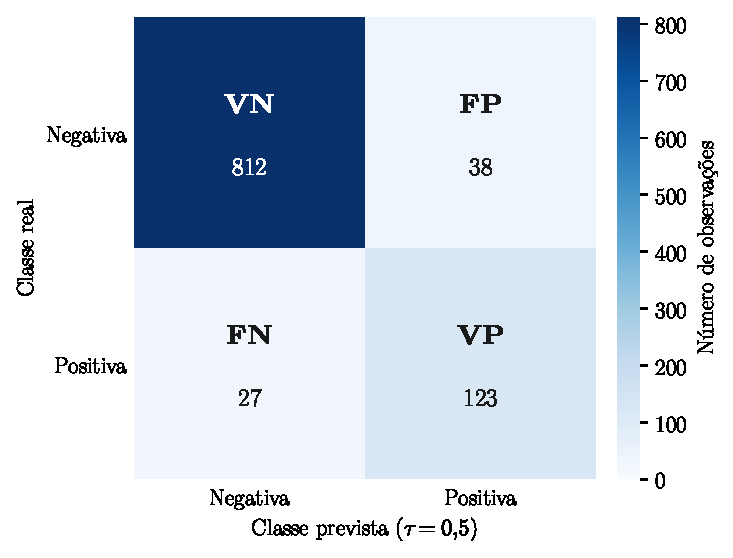
\includegraphics[width=0.65\textwidth]{figuras/matriz_confusao}
  \label{fig:matriz_confusao}
  \fonte{Elaborada pelo autor (\ano).}
\end{figure}

A Figura~\ref{fig:f1_classificadores} compara o \textit{F1-score} (Equação~\eqref{eq:f1}) dos quatro classificadores avaliados nas $k = 5$ partições da validação cruzada. As barras indicam a média, as hastes o desvio-padrão e os pontos o valor obtido em cada partição.

\begin{figure}[H]
  \centering
  \caption{Desempenho dos classificadores segundo o \textit{F1-score} na validação cruzada}
  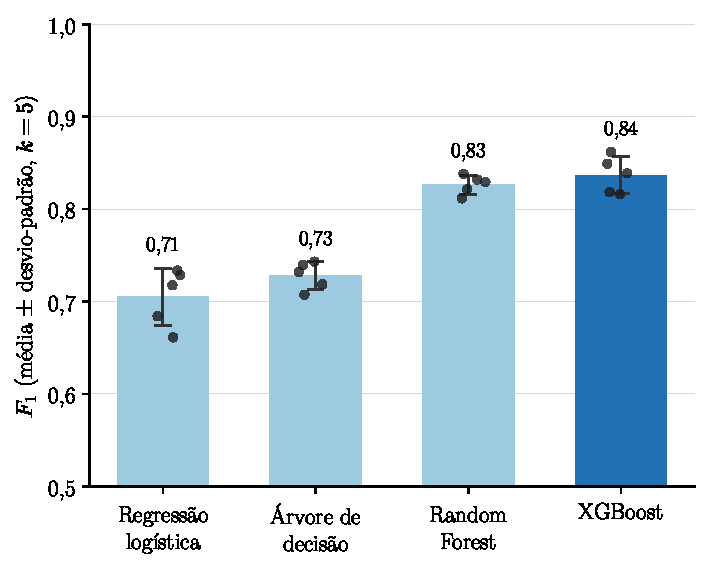
\includegraphics[width=0.75\textwidth]{figuras/f1_classificadores}
  \label{fig:f1_classificadores}
  \fonte{Elaborada pelo autor (\ano).}
\end{figure}

% Exemplo 7: figuras lado a lado (dois minipage dentro de um único figure)
% Cada minipage recebe seu próprio \caption, \label e \fonte, e cada imagem
% é numerada como uma figura independente. A soma das larguras (0.48 + 0.48)
% deve ficar abaixo de 1\textwidth; o \hfill distribui o espaço restante.
% Não deixe linha em branco entre os minipage, ou eles serão empilhados.
% A mesma altura máxima (height + keepaspectratio) nas duas imagens alinha
% as fontes na mesma linha, mesmo com proporções diferentes.
As Figuras~\ref{fig:matriz_confusao_lado} e~\ref{fig:f1_classificadores_lado} apresentam, lado a lado, a matriz de confusão e o desempenho comparativo dos classificadores, o que permite relacionar a distribuição dos erros do melhor modelo à sua posição relativa entre as alternativas avaliadas.

\begin{figure}[H]
  \centering
  \begin{minipage}[t]{0.48\textwidth}
    \centering
    \caption{Matriz de confusão do classificador XGBoost}
    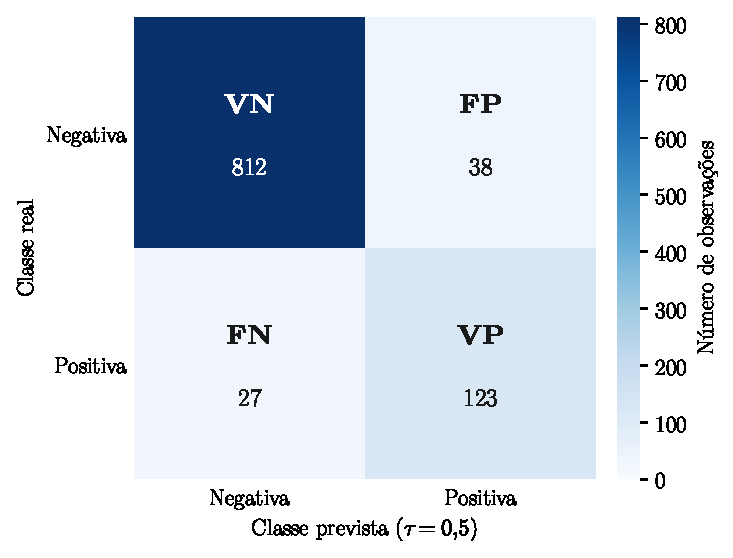
\includegraphics[width=\linewidth,height=0.74\linewidth,keepaspectratio]{figuras/matriz_confusao}
    \label{fig:matriz_confusao_lado}
    \fonte{Elaborada pelo autor (\ano).}
  \end{minipage}%
  \hfill
  \begin{minipage}[t]{0.48\textwidth}
    \centering
    \caption{\textit{F1-score} dos classificadores na validação cruzada}
    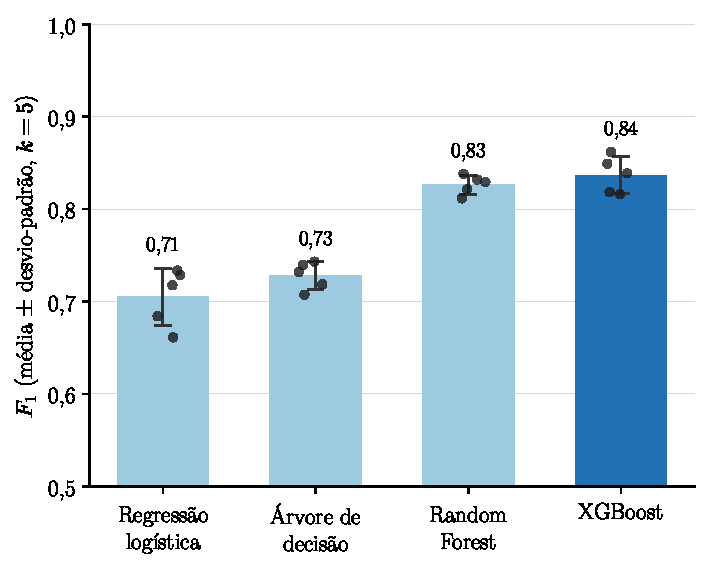
\includegraphics[width=\linewidth,height=0.74\linewidth,keepaspectratio]{figuras/f1_classificadores}
    \label{fig:f1_classificadores_lado}
    \fonte{Elaborada pelo autor (\ano).}
  \end{minipage}
\end{figure}

\section{Aspectos éticos}
\label{sec:aspectos_eticos}
Pesquisas que envolvem seres humanos, direta ou indiretamente (questionários, entrevistas, dados pessoais), devem ser submetidas ao Comitê de Ética em Pesquisa por meio da Plataforma Brasil, em conformidade com as Resoluções CNS n.º 466/2012 e n.º 510/2016. Nesse caso, esta seção deve informar a situação da submissão, os procedimentos de obtenção do Termo de Consentimento Livre e Esclarecido e as medidas de anonimização e proteção de dados previstas, em observância à Lei Geral de Proteção de Dados.

\textbf{A Resolução CNS n.º 510/2016 (art. 1º, parágrafo único, inciso I) dispensa de registro e avaliação pelo sistema CEP/CONEP a pesquisa de opinião pública com participantes não identificados, entendida como consulta pontual na qual o participante expressa preferência, avaliação ou o sentido que atribui a temas, organizações, produtos ou serviços. O enquadramento exige que não haja possibilidade de identificação em nenhuma etapa da coleta (sem registro de e-mail, \textit{login} ou combinações de variáveis que permitam reidentificação).} Instrumentos com escalas de mensuração voltados ao teste de relações entre construtos, ou que abordem condutas sensíveis, tendem a não se enquadrar nessa dispensa. Quando o enquadramento for adotado, esta seção deve indicar o inciso que o fundamenta, descrever as garantias de anonimato e apresentar o termo de esclarecimento exibido ao respondente, preferencialmente acompanhado de manifestação formal do CEP institucional sobre a dispensa. Caso a pesquisa não envolva seres humanos, essa condição deve ser declarada e justificada.

\section{Delimitações e limitações do estudo}
\label{sec:limitacoes}
As delimitações expressam escolhas deliberadas do pesquisador quanto ao escopo (recorte temporal, setor, população, bases consultadas). As limitações, por sua vez, decorrem de restrições metodológicas, de dados ou de infraestrutura que escapam ao seu controle. Na etapa de qualificação, ambas são previstas, e não verificadas, e sua explicitação orienta o alcance interpretativo dos achados, prevenindo generalizações indevidas. Essas fronteiras também funcionam como subsídio para o delineamento de pesquisas futuras.

\begin{enumerate}
  \item \preencher{Delimitação ou limitação 1}.
  \item \preencher{Delimitação ou limitação 2}.
  \item \preencher{Delimitação ou limitação 3}.
  \item \preencher{Delimitação ou limitação 4}.
\end{enumerate}
% ==============================================================================
% CAPÍTULO 4: RESULTADOS
% O título muda conforme a etapa (\titresultados, definido em main.tex):
% "Resultados preliminares" na qualificação e "Resultados e discussão" na Defesa.
% ==============================================================================
\chapter{\titresultados}
\label{ch:analise_discussao}
\begin{resumocapitulo}
  Aqui deve ser incluído um resumo do capítulo, descrevendo, de forma reduzida, os achados até o momento, de acordo com os objetivos propostos com o limite de 200 palavras.
\end{resumocapitulo}

\preencher{A análise e a discussão dos resultados preliminares têm como finalidade examinar e contextualizar criticamente os primeiros achados empíricos obtidos na investigação, confrontando-os com o quadro teórico previamente estabelecido. O seu papel estrutural é interpretar o comportamento das variáveis, padrões emergentes ou evidências parciais à luz da literatura e dos objetivos da pesquisa, avaliando a consistência dos modelos analíticos aplicados. Essa seção permite diagnosticar a adequação dos protocolos metodológicos em curso, subsidiar eventuais ajustes analíticos e antecipar as tendências que orientarão a consolidação das conclusões finais da dissertação. Apagar este texto de instrução após a redação da seção.}

\section{Visão geral}
\label{sec:visao_geral_resultados}
Descrever uma síntese do que será tratado no capítulo, incluindo os objetivos específicos e os resultados preliminares obtidos. A visão geral deve fornecer ao leitor um panorama dos achados, destacando como cada resultado contribui para responder à pergunta de pesquisa e alcançar os objetivos propostos. Podem ser utilizadas outras subseções para organizar os resultados por objetivo específico, por construto teórico ou por tipo de análise realizada.

Exemplo de inserção de tabela com os resultados numéricos. A Tabela~\ref{tab:exemplo} apresenta resultados numéricos aleatórios. Substituir com seus dados.
\begin{table}[H]
  \centering
  \caption{Exemplo de tabela com apresentação de dados numéricos}
  \label{tab:exemplo}
  \begin{tabular*}
    {\linewidth}
    {@{\extracolsep{\fill}} l c}
    \hline \textbf{Métrica} & \textbf{Valor} \\ \hline Acurácia (\textit{accuracy}) & 0,51 \\ Precisão (\textit{precision}) & 0,50 \\ Revocação (\textit{recall}) & 0,96 \\ \textit{F1-score} & 0,66 \\ \hline
  \end{tabular*}
  \fonte{Elaborada pelo autor (\ano).}
\end{table}

\ifdefesa
  % ==============================================================================
% CAPÍTULO 5: CONCLUSÃO (somente na Defesa)
% Substitui automaticamente o capítulo "Planos para a continuidade do trabalho"
% quando \Tipoexame{Defesa} (ver main.tex). Também pode ser intitulado
% "Considerações finais".
% A conclusão NÃO é um resumo do trabalho (manual, cap. 3, item 3): é a síntese
% dos resultados à luz da pergunta de pesquisa e dos objetivos.
% Não se introduzem dados, citações ou argumentos novos neste capítulo.
% ==============================================================================
\chapter{Conclusão}
\label{ch:conclusao}

\preencher{A conclusão tem como finalidade responder explicitamente à pergunta de pesquisa e demonstrar em que medida os objetivos foram atingidos, com base nos resultados apresentados no Capítulo~\ref{ch:analise_discussao}. Apagar este texto de instrução após a redação do capítulo.}

\section{Resposta à pergunta de pesquisa}
\label{sec:resposta_pergunta}
Retomar a \hyperref[perg:principal]{Pergunta de Pesquisa} e respondê-la de forma direta, indicando como cada objetivo específico (Seção~\ref{subsec:objetivos_especificos}) foi atendido e com quais evidências. Convém seguir a mesma ordem dos objetivos, o que permite ao leitor verificar a correspondência entre o que foi proposto e o que foi alcançado.

\section{Contribuições teóricas e práticas}
\label{sec:contribuicoes_finais}
Explicitar o que o trabalho acrescenta à literatura e à prática, confrontando o resultado obtido com as contribuições esperadas anunciadas na Seção~\ref{sec:contribuicoes}. Contribuições não confirmadas também devem ser reconhecidas.

\section{Limitações}
\label{sec:limitacoes_finais}
Apresentar as limitações efetivamente verificadas ao longo da pesquisa, retomando as previstas na Seção~\ref{sec:limitacoes} e indicando de que modo elas restringem o alcance das conclusões.

\section{Trabalhos futuros}
\label{sec:trabalhos_futuros}
Indicar desdobramentos concretos, preferencialmente derivados das limitações identificadas, e não sugestões genéricas.
  % Defesa
\else
  % ==============================================================================
% CAPÍTULO 5: PLANOS PARA A CONTINUIDADE DO TRABALHO
% ==============================================================================
\chapter{Planos para a continuidade do trabalho}
\label{ch:plano_trabalho}
Os planos para a continuidade do trabalho têm como finalidade formalizar a transição entre a etapa atual e a defesa final da dissertação, detalhando as ações técnicas, empíricas e analíticas que ainda precisam ser executadas. O seu papel estrutural é apresentar um planejamento operacional exequível, delimitando a coleta complementar de dados, o refinamento dos modelos estatísticos ou computacionais, a redação dos capítulos conclusivos e o cronograma de atividades até a conclusão do mestrado. Essa seção demonstra a viabilidade do projeto e evidencia a capacidade do pesquisador de cumprir o cronograma acadêmico dentro dos prazos regulamentares.

\section{Atividades previstas até a qualificação}
\label{sec:atividades_ate_qualificacao}
A seção de atividades previstas até a qualificação tem como finalidade delimitar o conjunto de tarefas científicas, técnicas e documentais necessárias para consolidar a maturidade teórica e metodológica do projeto antes de sua primeira avaliação formal por banca examinadora. O seu papel estrutural é estabelecer o roteiro preparatório do mestrando, detalhando o fechamento da revisão de literatura, o delineamento dos protocolos experimentais, a realização de provas de conceito (POC) ou coletas preliminares, a submissão ao Comitê de Ética (quando aplicável) e a redação do texto de qualificação. Esse mapeamento atesta a consistência do percurso inicial e assegura que a pesquisa atinja o estágio de desenvolvimento exigido para receber as contribuições críticas da comissão julgadora.

\section{Atividades previstas da qualificação à defesa}
\label{sec:atividades_ate_defesa}
Esta seção tem como finalidade desdobrar analítica e operacionalmente as atividades posteriores à qualificação, transformando marcos temporais em planos de ação concretos. Para cada etapa, devem ser especificados os métodos, insumos, ferramentas computacionais, critérios de validação e entregáveis esperados, incluindo a incorporação dos apontamentos da banca, a coleta e análise dos dados empíricos, a submissão de artigo científico, a disponibilização de código e dados em repositório aberto e a redação final. Essa discriminação mitiga riscos de execução e assegura que a transição entre as etapas empíricas e a redação conclusiva ocorra com rigor e conformidade temporal.

\section{Cronograma}
\label{sec:cronograma}
O Quadro~\ref{qua:cronograma} consolida as atividades descritas nas seções anteriores até a defesa final da dissertação.

\begin{quadros}[H]
  \centering
  \caption{Plano de trabalho para conclusão da dissertação no ano de 2027}
  \label{qua:cronograma}
  \scriptsize
  \singlespacing
  \setlength{\tabcolsep}{5pt}
  \renewcommand{\arraystretch}{1.2}
  % Altura uniforme de todas as linhas (ajustar se alguma atividade ocupar 3 linhas)
  \newlength{\alturalinha}
  \setlength{\alturalinha}{2.8em}
  % Célula de atividade com altura fixa e texto centralizado verticalmente
  \newcommand{\ativ}[1]{\parbox[c][\alturalinha][c]{0.36\linewidth}{\raggedright #1}}
  \begin{tabular}{|c|l|c|c|c|c|c|c|c|c|c|c|c|c|}
    \hline
    \multicolumn{2}{|c|}{\parbox[c][1.8em][c]{0pt}{}}                          &
    \multicolumn{12}{c|}{\textbf{2027}}                                                                                                                                                                                                                                                                         \\ \hline

    \textbf{\textit{n}}                                                        &
    \parbox[c][\alturalinha][c]{0.36\linewidth}{\centering\textbf{ATIVIDADES}} &
    \textbf{01}                                                                & \textbf{02}                                                                        & \textbf{03} & \textbf{04} & \textbf{05} & \textbf{06} & \textbf{07} & \textbf{08} & \textbf{09} & \textbf{10} & \textbf{11} & \textbf{12} \\ \hline

    1                                                                          & \ativ{Integração inicial de dados e desenvolvimento da POC}                        &
                                                                               & \mes                                                                               & \mes        & \mes        &             &             &             &             &             &             &             &             \\ \hline

    2                                                                          & \ativ{Consolidação da versão preliminar e \textbf{Pré-Qualificação}}               &
                                                                               &                                                                                    &             & \mes        & \mes        &             &             &             &             &             &             &             \\ \hline

    3                                                                          & \ativ{Refinamento teórico-metodológico e redação para o exame de qualificação}     &
                                                                               &                                                                                    &             &             &             & \mes        & \mes        &             &             &             &             &             \\ \hline

    4                                                                          & \ativ{\textbf{Exame de Qualificação}}                                              &
                                                                               &                                                                                    &             &             &             &             &             & \mes        &             &             &             &             \\ \hline

    5                                                                          & \ativ{Coleta e extração sistemática de dados empíricos}                            &
                                                                               &                                                                                    &             &             &             &             &             & \mes        & \mes        & \mes        &             &             \\ \hline

    6                                                                          & \ativ{Implementação dos apontamentos da banca de qualificação}                     &
                                                                               &                                                                                    &             &             &             &             &             &             & \mes        &             &             &             \\ \hline

    7                                                                          & \ativ{Processamento e análise dos dados}                                           &
                                                                               &                                                                                    &             &             &             &             &             &             & \mes        & \mes        &             &             \\ \hline

    8                                                                          & \ativ{Finalização e \textbf{Submissão de Artigo Científico}}                       &
                                                                               &                                                                                    &             &             &             &             &             &             &             &             & \mes        &             \\ \hline

    9                                                                          & \ativ{Consolidação dos resultados, redação final e revisão textual da dissertação} &
                                                                               &                                                                                    &             &             &             &             &             &             &             & \mes        & \mes        & \mes        \\ \hline

    10                                                                         & \ativ{Disponibilização do repositório OSF com código e dados abertos}              &
                                                                               &                                                                                    &             &             &             &             &             &             &             &             &             & \mes        \\ \hline

    11                                                                         & \ativ{\textbf{Defesa da Dissertação}}                                              &
                                                                               &                                                                                    &             &             &             &             &             &             &             &             &             & \mes        \\ \hline
  \end{tabular}

  \fonte{Elaborado pelo autor (\ano).}
\end{quadros}
     % Pré-Qualificação e Qualificação
\fi

% ==============================================================================
% DECLARAÇÃO DE USO DE IA E ELEMENTOS PÓS-TEXTUAIS
% Títulos sem indicativo numérico, centralizados
% ==============================================================================
\postextual

% ==============================================================================
% DECLARAÇÃO DE USO DE IA GENERATIVA
% Título sem indicativo numérico (centralizado), após o corpo textual e antes
% das Referências. Manter somente os itens efetivamente aplicáveis.
% ==============================================================================
\chapter*{Declaração de uso de IA generativa}
\phantomsection
\addcontentsline{toc}{chapter}{Declaração de uso de IA generativa}
\markboth{DECLARAÇÃO DE USO DE IA GENERATIVA}{}
\label{ch:declaracao_ia_generativa}
A declaração de uso de IA generativa tem como finalidade formalizar a integridade ética, o rigor metodológico e a transparência científica do trabalho, documentando a extensão da intervenção de ferramentas algorítmicas ao longo do processo de pesquisa e redação. O seu papel estrutural é discriminar com precisão os modelos e plataformas empregados (especificando versões, parâmetros ou finalidades de suporte), delimitar as tarefas assistidas (como revisão estilística, estruturação preliminar de código, tradução ou exploração conceitual) e atestar a primazia da autoria humana. Esse registro assegura que a responsabilidade crítica, analítica e epistemológica sobre as conclusões, a verificação de alucinações e a exatidão das referências permaneçam integralmente sob o domínio do autor, alinhando a dissertação às diretrizes de governança ética e integridade acadêmica estabelecidas pela comunidade científica e pelas agências de fomento.

Para cada intervenção mediada por modelos computacionais, reportam-se: a \textit{localização} (em que proposições ou seções a ferramenta introduziu, selecionou ou modificou conteúdo material), a \textit{extensão} (a natureza e o nível da operação realizada) e a \textit{verificação} (o procedimento pelo qual o autor examinou criticamente o resultado antes de assumir a responsabilidade pela sua incorporação).

\section*{Ferramentas utilizadas}
% Manter apenas os itens correspondentes às ferramentas efetivamente utilizadas.
% Repetir o modelo adequado quantas vezes forem necessárias.
\begin{itemize}
  % Modelo 1: execução local ou em rede local
  \item \textbf{\preencher{nome e versão do modelo}} (\preencher{empresa}), executado em infraestrutura computacional \preencher{local, na própria estação de trabalho, ou em servidor da rede local institucional} sob o ambiente \textit{\preencher{nome e versão do ambiente de execução, por exemplo, llama.cpp, Ollama ou LM Studio}}, sem transmissão de dados ou telemetria para servidores externos, durante sessões conduzidas em \preencher{mês e ano}.

        % Modelo 2: acesso por interface de chat hospedada pelo fornecedor
  \item \textbf{\preencher{nome e versão do modelo}} (\preencher{empresa}), acessado pela interface de chat \textit{\preencher{nome da plataforma, por exemplo, claude.ai, chatgpt.com ou gemini.google.com}}, em plano \preencher{gratuito, individual ou institucional}, com mecanismo de busca na web \preencher{ativado ou desativado}\preencher{, se ativado: para averiguação de registros externos} e com o uso dos dados para treinamento do modelo \preencher{habilitado ou desabilitado}, durante sessões conduzidas em \preencher{mês e ano}.
\end{itemize}

\section*{Intervenções e sua incidência sobre as afirmações}
As intervenções realizadas restringiram-se ao suporte linguístico e à verificação documental, não incidindo de forma material sobre as afirmações substantivas que fundamentam as conclusões do trabalho:
\begin{enumerate}
  \item \textbf{Sugestões de concisão e clareza textual} (\preencher{nome e versão}).
        \textit{Localização:} intervenções pontuais e dispersas ao longo \preencher{das seções ou capítulos, com a respectiva numeração}.
        \textit{Extensão:} reformulação estilística e ajuste sintático de orações preexistentes.
        \textit{Verificação:} as sugestões foram incorporadas pelo autor unicamente quando preservaram de modo estrito o escopo inferencial e a qualificação das premissas originais, tendo sido descartadas quaisquer formulações que alterassem a força das alegações.

  \item \textbf{Conferência de metadados bibliográficos e fontes} (\preencher{nome e versão}).
        \textit{Localização:} seção de Referências e confrontação de citações no texto.
        \textit{Extensão:} validação de identificadores persistentes (DOIs), volume, número, intervalos de paginação e correspondência com fontes primárias.
        \textit{Verificação:} cada entrada bibliográfica e metadado sugerido foram conferidos individualmente pelo autor, diretamente junto aos repositórios e às bases originais indexadas.
\end{enumerate}

\section*{Delimitação da autoria e produção não mediada por IA}
A formulação do problema de investigação, \preencher{tese, hipótese ou argumento central do trabalho}, \preencher{distinções teóricas, modelos conceituais ou taxonomias propostas}, \preencher{critérios, categorias analíticas ou procedimentos metodológicos definidos pelo autor} e \preencher{tabelas, figuras ou quadros conceituais de autoria própria, com a respectiva numeração} foram idealizados, estruturados e desenvolvidos de forma autônoma pelo autor, antes do emprego de quaisquer ferramentas computacionais.

A ferramenta \preencher{nome e versão} foi empregada na etapa de \preencher{busca, triagem ou seleção} da literatura, cabendo ao autor a verificação integral das fontes e a decisão final de inclusão.

\section*{Comandos textuais utilizados (\textit{Prompts})}
\begin{itemize}
  \item \textbf{Sugestões de concisão e clareza} (\preencher{nome e versão}):\\
        \textit{``Sugira opções de reformulação sintática para aumentar a concisão e a clareza do excerto a seguir, preservando integralmente o alcance das afirmações e sem introduzir novas proposições: [texto].''}

  \item \textbf{Conferência de metadados bibliográficos e fontes} (\preencher{nome e versão}):\\
        \textit{``Examine a lista de referências anexa e valide a exatidão dos respectivos metadados bibliográficos (especificamente autoria, título, periódico, ano, volume, número, páginas e DOI) e sua correspondência com os registros publicados: [lista de referências].''}
\end{itemize}


% Estilo ABNT autor-data com ponto e vírgula entre autores (NBR 10520:2023)
\bibliographystyle{config/abntex2-alf-uninove}
\bibliography{config/abnt-opcoes,pos-textuais/referencias}  % obrigatório

% Apêndices (elaborados pelo autor)
\apendice{Expressões de busca da revisão sistemática}
\label{ap:ap_string}

\subsection*{Scopus}

\begin{quadros}[!ht]
  \caption{Expressão de busca aplicada na base Scopus}
  \label{qua:string_scopus}
\begin{lstlisting}[style=busca]
TITLE-ABS-KEY(
  ("traffic congestion" OR "traffic flow" OR "traffic speed")
  AND (forecast* OR predict*)
  AND ("machine learning" OR "gradient boosting" OR
       "random forest" OR "XGBoost" OR "deep learning")
  AND (explainab* OR interpretab* OR "SHAP")
)
AND PUBYEAR > 2014 AND PUBYEAR < 2026
AND LANGUAGE(English) AND DOCTYPE(ar)
\end{lstlisting}
  {\footnotesize\singlespacing Data da busca: 12/05/2025. Registros recuperados: 412.\par}
  \fonte{Elaborado pela autora (\ano).}
\end{quadros}

\subsection*{Web of Science}

\begin{quadros}[!ht]
  \caption{Expressão de busca aplicada na base Web of Science}
  \label{qua:string_wos}
\begin{lstlisting}[style=busca]
TS=(
  ("traffic congestion" OR "traffic flow" OR "traffic speed")
  AND (forecast* OR predict*)
  AND ("machine learning" OR "gradient boosting" OR
       "random forest" OR "XGBoost" OR "deep learning")
  AND (explainab* OR interpretab* OR "SHAP")
)
\end{lstlisting}
  {\footnotesize\singlespacing Filtros: período (2015--2025), tipo (artigo), idioma (inglês). Data da busca: 12/05/2025. Registros recuperados: 287.\par}
  \fonte{Elaborado pela autora (\ano).}
\end{quadros}

\begin{orientacao}[Inclusão de outras bases de dados]
  As bases Scopus e Web of Science são apresentadas apenas como exemplo. Inclua todas as bases efetivamente consultadas na revisão, como IEEE Xplore, ACM Digital Library, ScienceDirect, PubMed, SciELO ou bases específicas da área, cada uma em sua própria subseção e em seu próprio quadro. Cada base tem sintaxe própria (campos, operadores e truncamentos), por isso a expressão deve ser transcrita exatamente como foi executada, e não apenas traduzida a partir da expressão da Scopus. Os conceitos e a lógica booleana, entretanto, devem ser equivalentes entre as bases, e eventuais diferenças precisam ser justificadas na Metodologia. Para cada base, registre a data da busca, os filtros aplicados e o número de registros recuperados. A soma desses números deve coincidir com o total informado na etapa de identificação do fluxo PRISMA. O Google Acadêmico pode ser usado como fonte complementar, mas não substitui as bases indexadas, porque seus resultados variam ao longo do tempo e não podem ser reproduzidos.
\end{orientacao}

% ------------------------------------------------------------------------------
% MODELO PARA NOVA BASE (copiar, descomentar e ajustar)
% Trocar o nome da base, o rótulo (qua:string_...), a expressão, os filtros,
% a data e o número de registros. Manter a expressão exatamente como foi
% executada na base, para que possa ser copiada do PDF e reaplicada.
% ------------------------------------------------------------------------------
% \subsection*{IEEE Xplore}
%
% \begin{quadros}[!ht]
%   \caption{Expressão de busca aplicada na base IEEE Xplore}
%   \label{qua:string_ieee}
% \begin{lstlisting}[style=busca]
% ("All Metadata":"traffic congestion" OR "All Metadata":"traffic flow")
% AND ("All Metadata":forecast* OR "All Metadata":predict*)
% AND ("All Metadata":"machine learning" OR "All Metadata":"deep learning")
% AND ("All Metadata":explainab* OR "All Metadata":"SHAP")
% \end{lstlisting}
%   {\footnotesize\singlespacing Filtros: período (2015--2025), tipo (artigo de periódico). Data da busca: dd/mm/aaaa. Registros recuperados: n.\par}
%   \fonte{Elaborado pelo(a) autor(a) (\ano).}
% \end{quadros}
\apendice{Dicionário de variáveis}
\label{ap:variaveis}

\begin{orientacao}[Dicionário de variáveis]
  O dicionário de variáveis documenta cada atributo da base utilizada na modelagem e permite que outro pesquisador compreenda, audite e reproduza o estudo. Liste todas as variáveis que entram no modelo, inclusive as derivadas (defasagens, médias móveis, indicadores calculados), e identifique a variável-alvo. Para cada uma, informe o tipo, a unidade ou o domínio de valores, a origem e, no caso das variáveis derivadas, a regra de cálculo. Essa informação é decisiva para afastar o vazamento de dados: uma variável derivada que use informação posterior ao instante da previsão invalida a avaliação do modelo. Se a base tiver muitas variáveis, agrupe-as por dimensão (temporal, meteorológica, operacional) ou divida o quadro em mais de uma página. No texto, cite o quadro antes de ele aparecer.
\end{orientacao}

O Quadro~\ref{qua:variaveis} descreve as variáveis da base de dados utilizada na modelagem, com a origem de cada uma. As variáveis derivadas foram calculadas apenas com informações disponíveis até o instante da previsão.

\begin{quadros}[H]
  \centering
  \caption{Dicionário de variáveis da base horária}
  \label{qua:variaveis}
  \small
  \singlespacing
  \setlength{\tabcolsep}{4pt}
  \renewcommand{\arraystretch}{1.3}
  \begin{tabular}{|l|c|c|l|l|}
    \hline
    \textbf{Variável} & \textbf{Tipo} & \textbf{Unidade} & \textbf{Descrição} & \textbf{Origem} \\ \hline
    \texttt{lentidao\_km}   & contínua   & km       & Extensão total de lentidão (alvo)    & CET-SP \\ \hline
    \texttt{lentidao\_lag1} & contínua   & km       & Lentidão observada na hora anterior  & Derivada \\ \hline
    \texttt{hora}           & discreta   & 0 a 23   & Hora do dia                          & Derivada \\ \hline
    \texttt{dia\_semana}    & categórica & 1 a 7    & Dia da semana                        & Derivada \\ \hline
    \texttt{feriado}        & binária    & 0 ou 1   & Indicador de feriado                 & Calendário oficial \\ \hline
    \texttt{precipitacao}   & contínua   & mm       & Precipitação acumulada na hora       & INMET \\ \hline
    \texttt{temperatura}    & contínua   & °C       & Temperatura média do ar              & INMET \\ \hline
    \texttt{ocorrencias}    & discreta   & contagem & Ocorrências viárias ativas           & CET-SP \\ \hline
    \texttt{eventos}        & binária    & 0 ou 1   & Evento de grande porte na cidade     & Agenda municipal \\ \hline
  \end{tabular}

  \fonte{Elaborado pela autora (\ano).}
  {\footnotesize\singlespacing Nota: CET-SP: Companhia de Engenharia de Tráfego de São Paulo; INMET: Instituto Nacional de Meteorologia. Variáveis derivadas: \texttt{lentidao\_lag1} corresponde a \texttt{lentidao\_km} defasada em uma hora; \texttt{hora} e \texttt{dia\_semana} foram extraídas do carimbo de data e hora do registro.\par}
\end{quadros}
\apendice{Trecho do código de modelagem}
\label{ap:codigo}

O código completo está disponível no repositório do projeto. O trecho a seguir apresenta o treinamento do modelo final e o cálculo dos valores SHAP.

\begin{lstlisting}[style=codigo, language=Python]
import pandas as pd
import shap
from xgboost import XGBRegressor

df = pd.read_parquet("dados/base_horaria.parquet")
treino = df[df["data_hora"] < "2024-01-01"]
teste = df[df["data_hora"] >= "2024-01-01"]

variaveis = ["hora", "dia_semana", "feriado", "lentidao_lag1",
             "precipitacao", "temperatura", "ocorrencias", "eventos"]

modelo = XGBRegressor(n_estimators=600, learning_rate=0.05,
                      max_depth=6, subsample=0.8, random_state=42)
modelo.fit(treino[variaveis], treino["lentidao_km"])

explicador = shap.TreeExplainer(modelo)
valores_shap = explicador.shap_values(teste[variaveis])
\end{lstlisting}


% Anexos (documentos de terceiros)
% % ==============================================================================
% ANEXO A: MODELO
% Documento NÃO elaborado pelo autor (lei, norma, parecer, instrumento validado
% de terceiros). Título: "ANEXO A – Título" (manual, cap. 4, item 4).
% Para incluir um PDF: \includepdf[pages=-,pagecommand={}]{anexos/arquivo.pdf}
% ==============================================================================
\anexo{Título do documento anexado}
\label{an:modelo}

Conteúdo do anexo ou inclusão do PDF correspondente.


\end{document}
